\chapter{Buildings and Structures}
\label{chapter:buildings}

\ifcoatlioan

The {\projectname} installation is spread through four buildings or structures: the ground-floor of the 84-cm telescope building; the shed; the access staircase and walkways; and the tower, platform, and enclosure. See Figure~\ref{figure:buildings-general}.

\fi

\ifddotioan

The {\projectname} installation is spread through four buildings or structures: the ground-floor of the 84-cm telescope building; the shed; the access walkways; and the tower, platform, and enclosure.

\fi

\begin{figure*}
\begin{center}
\includegraphics[height=0.7\linewidth]{figures/buildings-general.jpg}
\end{center}
\caption{The COATLI/OAN and DDOTI/OAN installations seen looking west. On the left is the COATLI/OAN shed, access staircase and walkways, tower, platform, and enclosure. In the middle is is 84-cm telescope building. On the right is the DDOTI/OAN tower, platform, enclosure, and shed. Photographer: Fernando Angeles.}
\label{figure:buildings-general}
\end{figure*}


\section{Civil Works}

\ifcoatlioan

The shed, access, and tower are constructed on a rock outcrop to the south-east of the 84-cm building. The outcrop rises to about 5 meters above the ground level at the 84-cm telescope. The buildings and structures were constructed in 2015--2016, the enclosure was installed in 2016, the enclosure was replaced in 2017, and the telescope column was significantly modified in 2018.

Figures~\ref{figure:buildings-drawing-2015-1} to \ref{figure:buildings-drawing-2015-5} show the 2015 design drawings for the shed, access staircase and walkways, and the concrete columns that support the platform and telescope. Figure  \ref{figure:buildings-drawing-astelco} shows the ASTELCO ARTS platform and the ASTELCO steel pillar mounted on the concrete columns. The center of rotation of the mount axes is 6.5 meters above the rock outcrop and about 11.5 meters above the ground at the 84-cm telescope. The long axis of the enclosure is oriented roughly ENE-WSW to match the shape of the rock outcrop.

The telescope concrete column originally had three parts, each square in cross section and tapering from 1.8, 1.2, and 0.6 meters to a side (see Figure~\ref{figure:buildings-drawing-2015-1}). In 2018, in response to concerns about stiffness, the column was modified and the upper two parts were reinforced to 1.4 meters to a side (see Figure \ref{figure:buildings-drawing-2018-1}). The steel pillar was also filled with concrete to the bottom of the upper holes. The platform floor was modified to accommodate the enlarged column and new support beams for the floor were designed, manufactured, and installed (see Figures \ref{figure:buildings-drawing-2018-2} and \ref{figure:buildings-drawing-2018-3}).

\begin{figure*}
\begin{center}
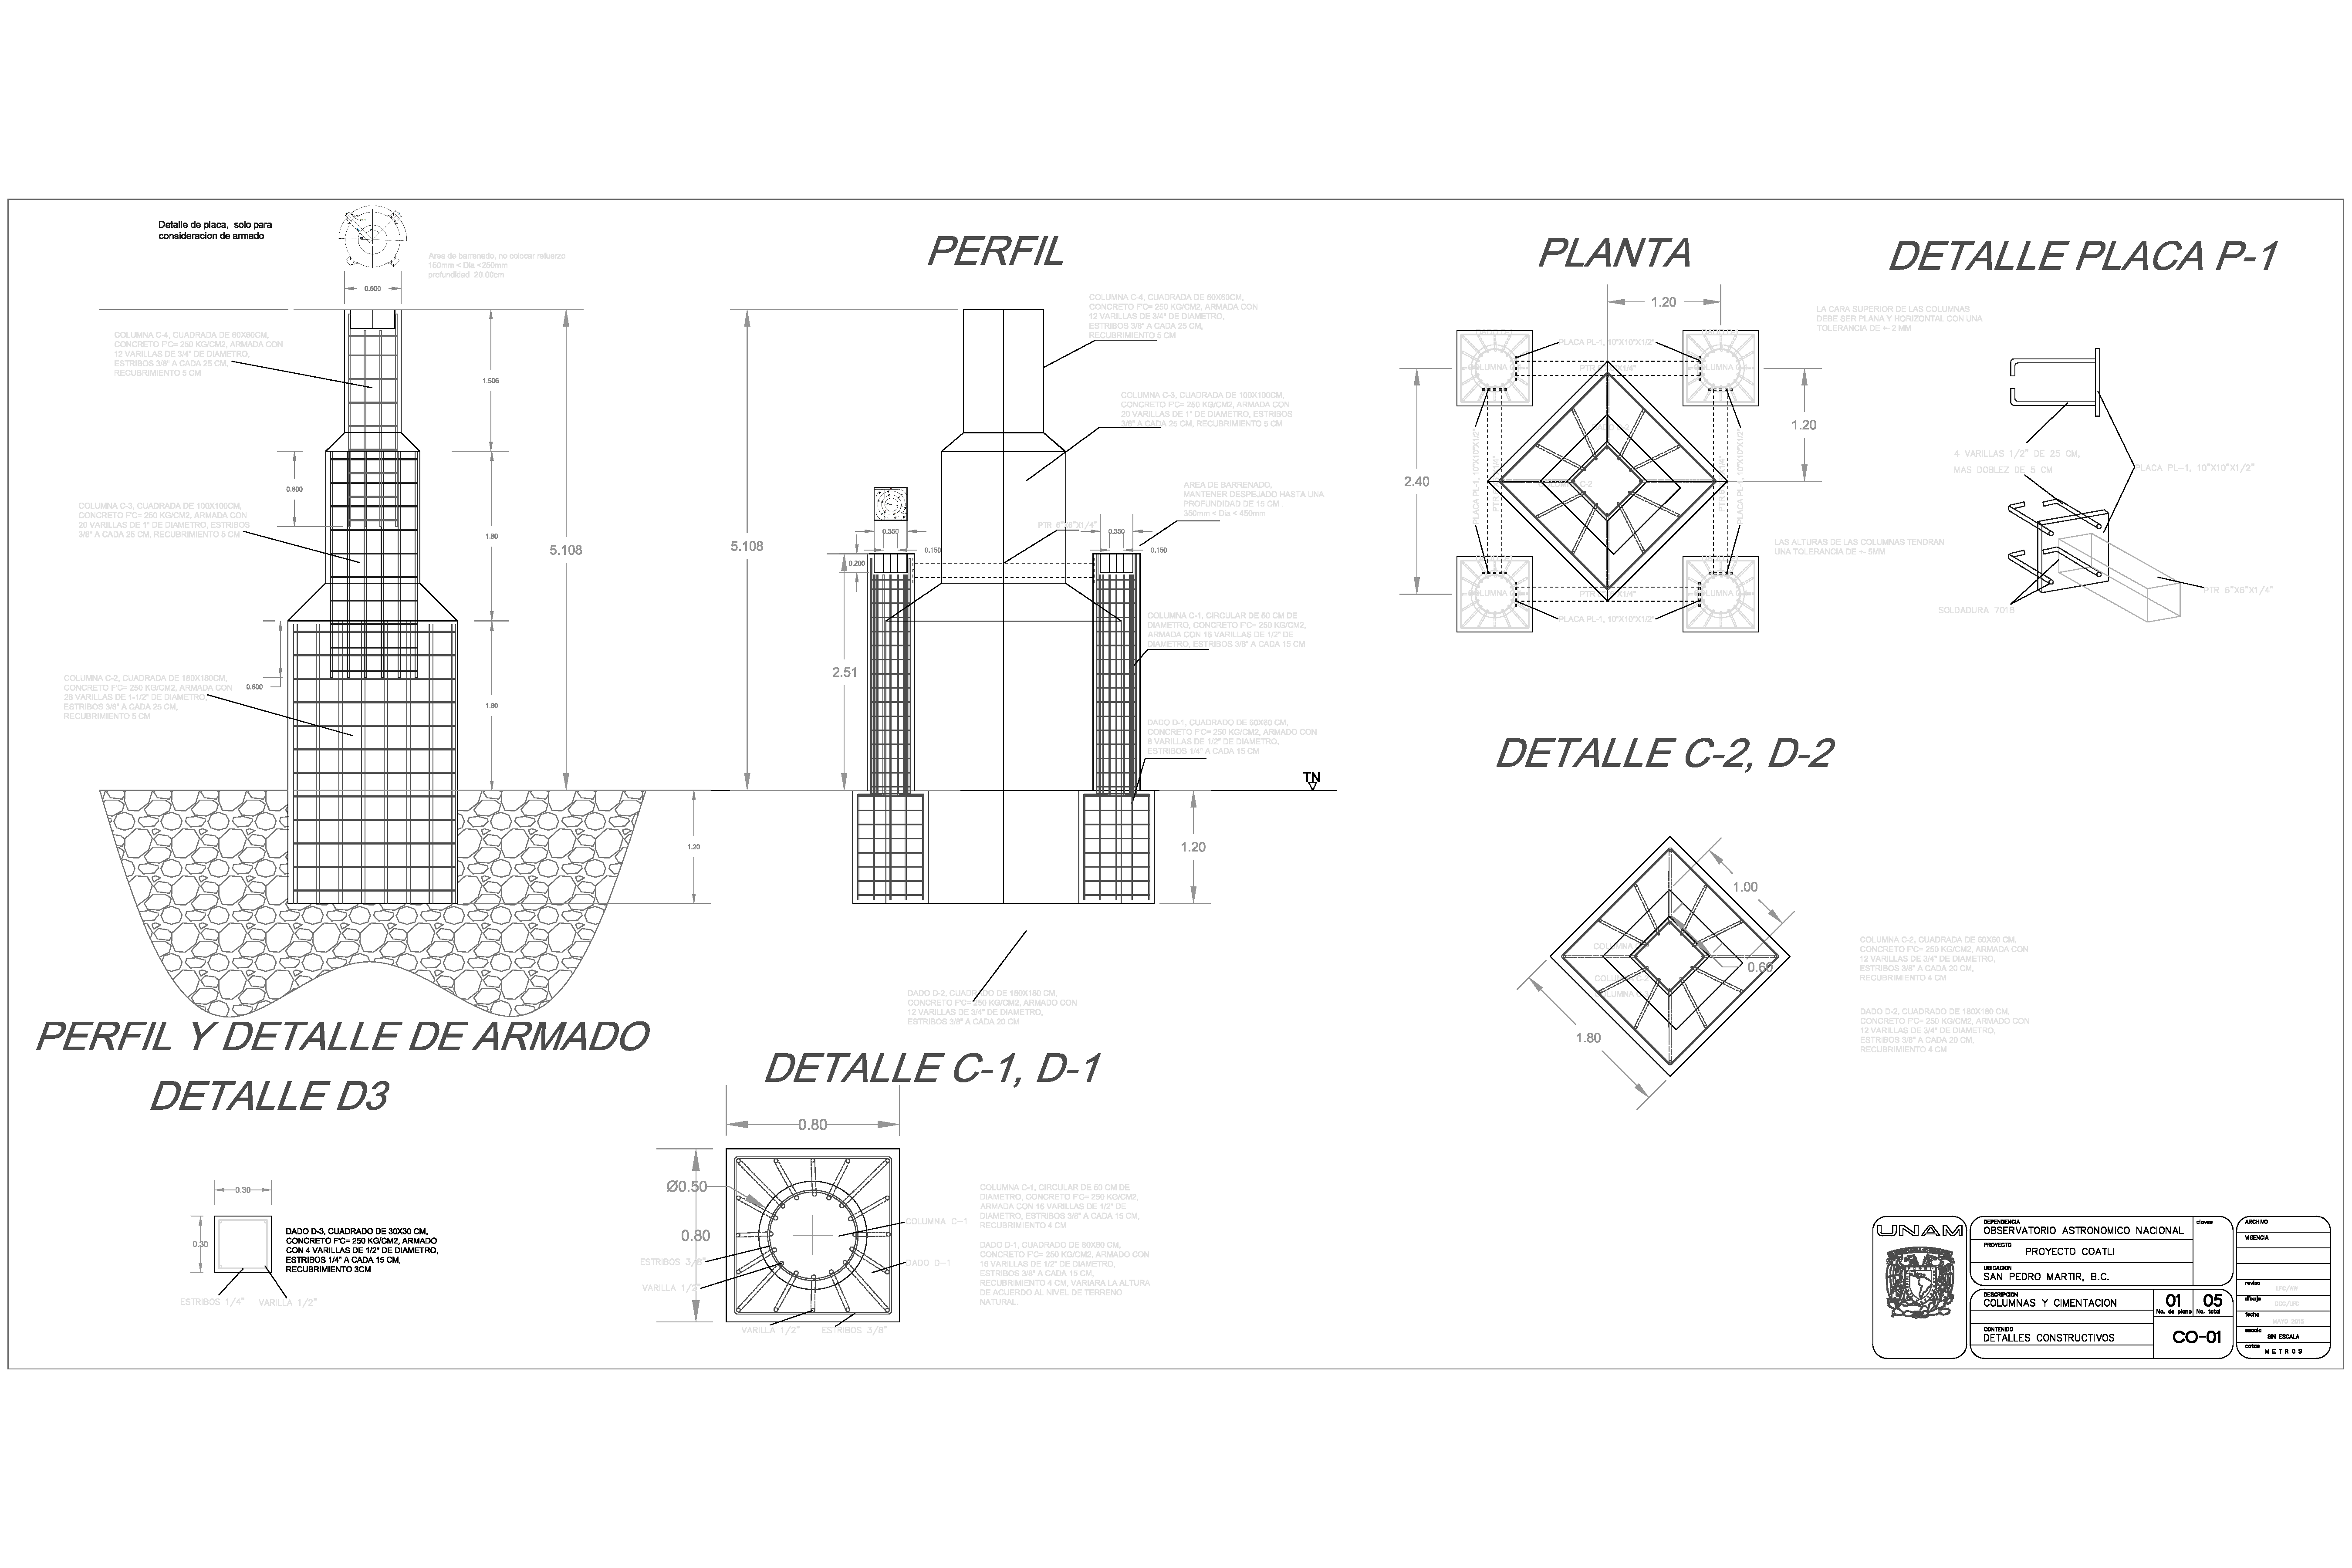
\includegraphics[height=0.95\linewidth,angle=90]{figures/buildings-coatli-drawing-2015-1.pdf}
\end{center}
\caption{{\projectname} original 2015 design drawing (1 of 5).}
\label{figure:buildings-drawing-2015-1}
\end{figure*}

\begin{figure*}
\begin{center}
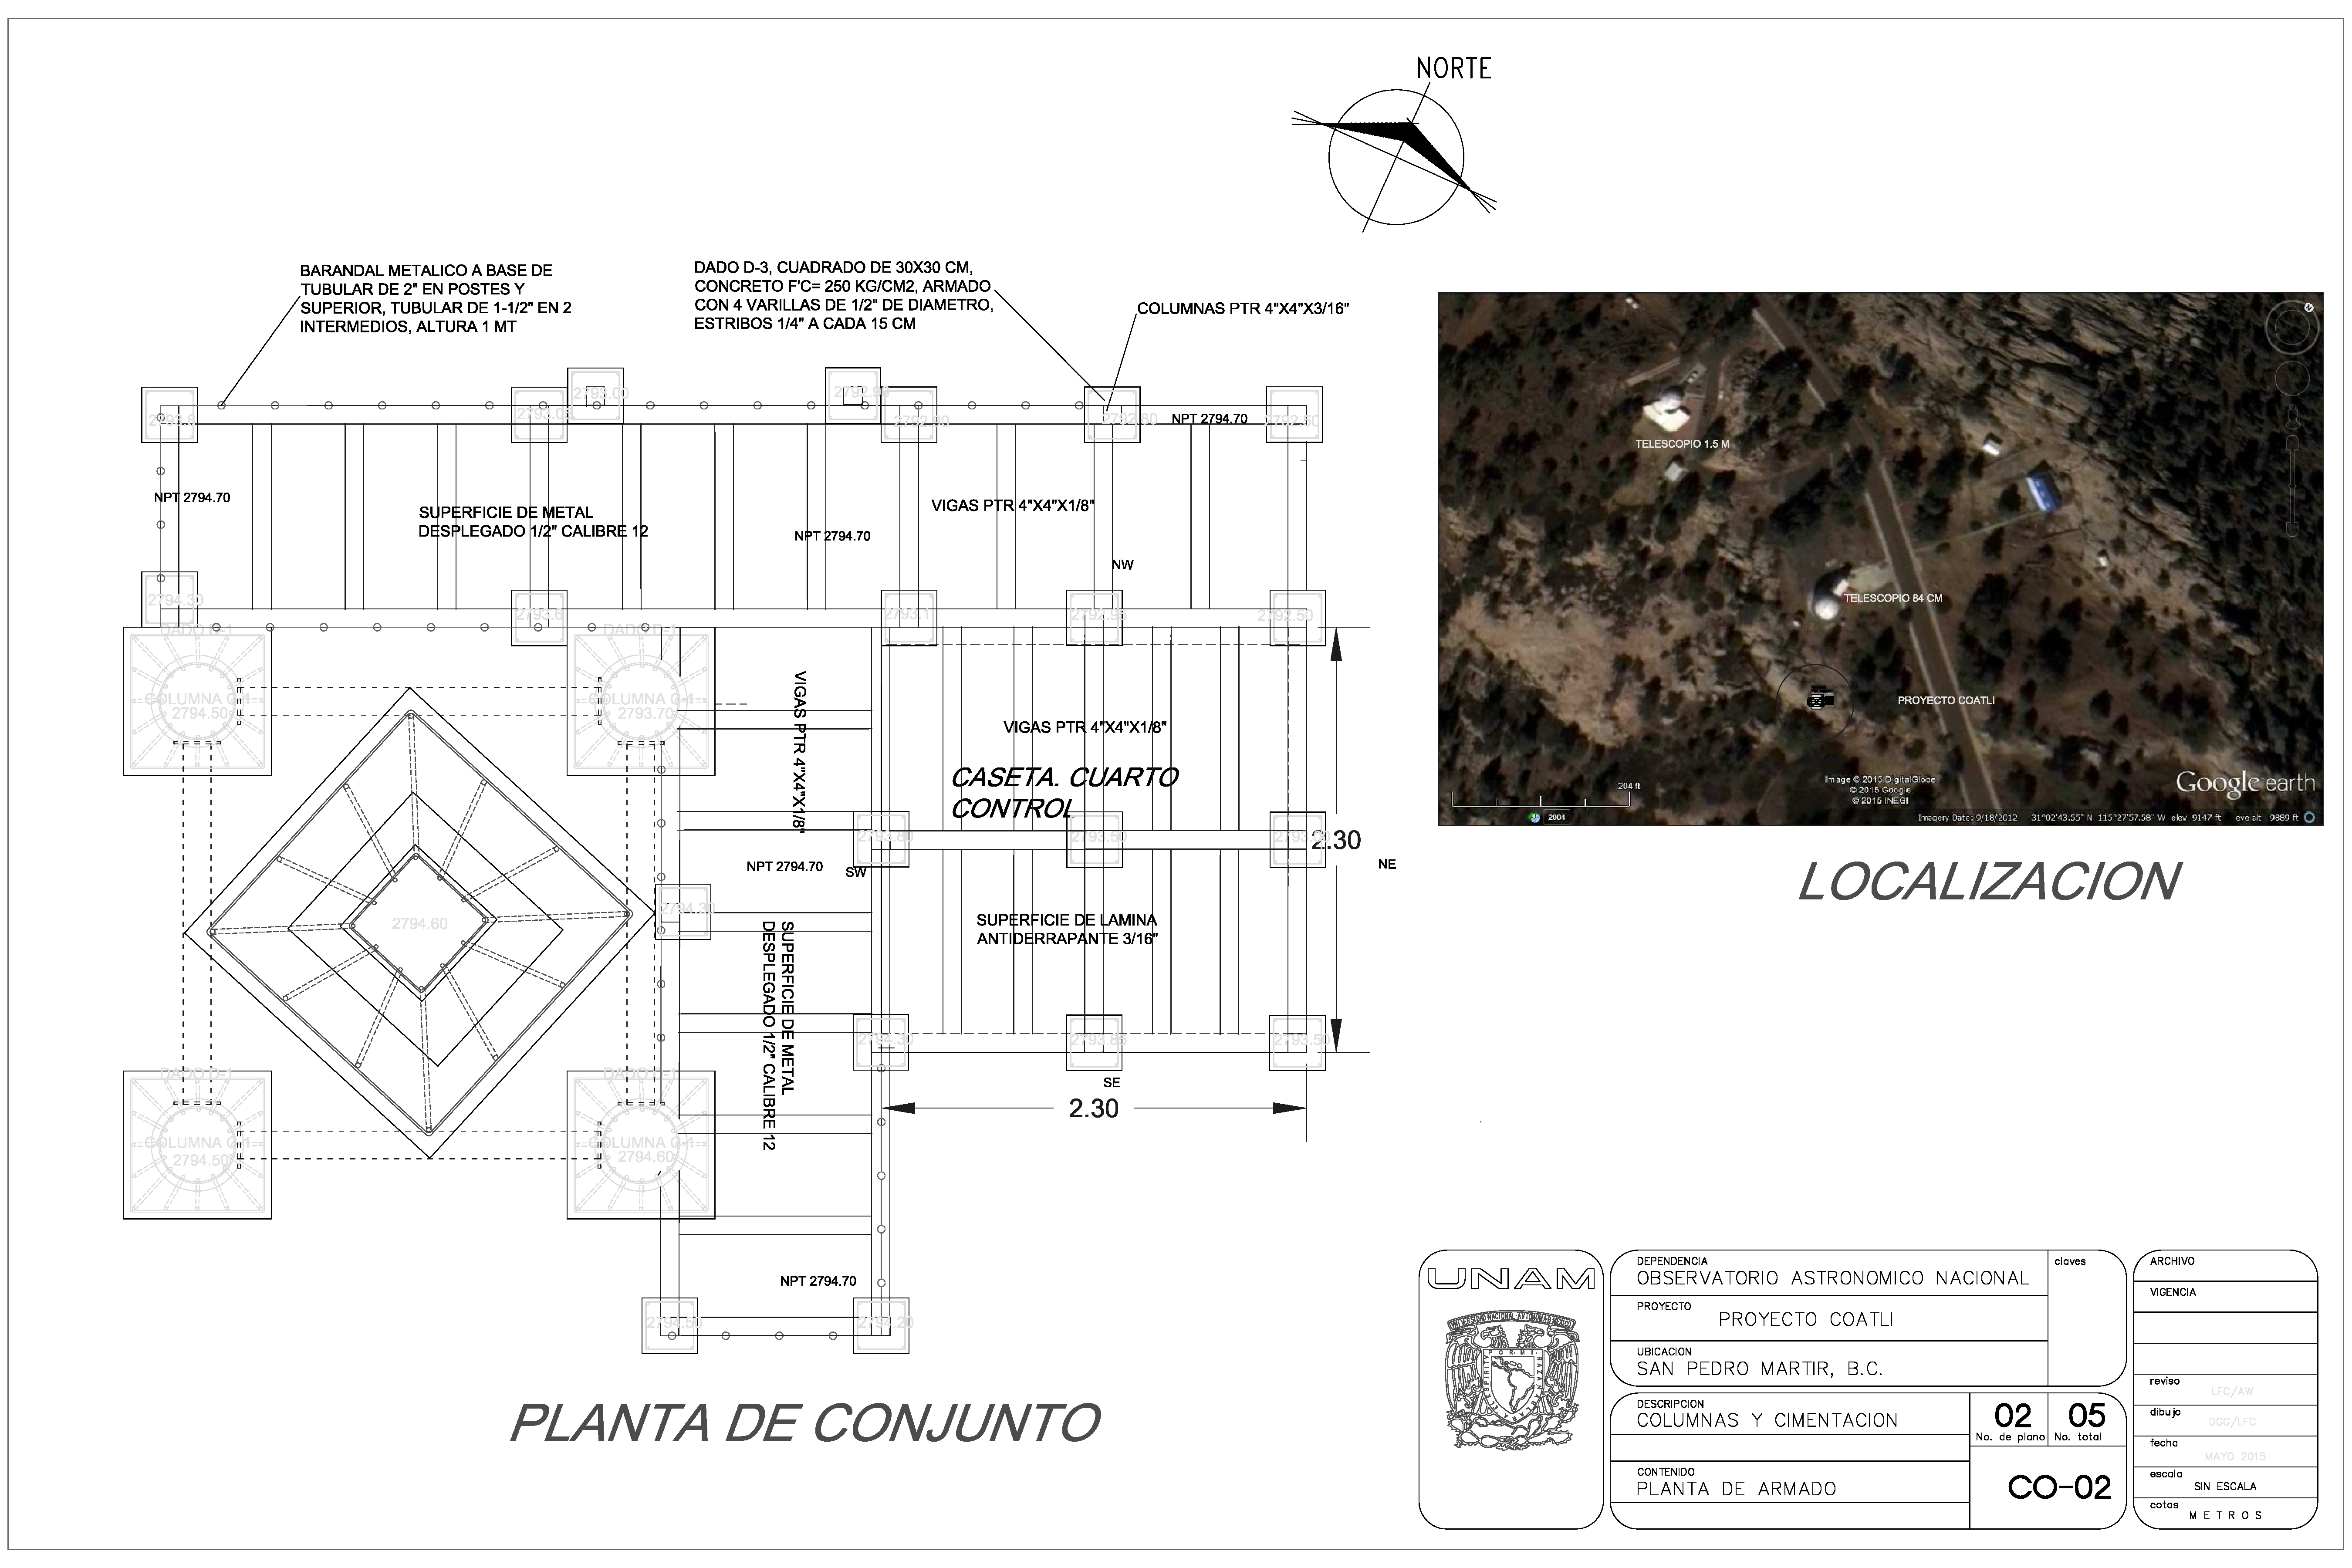
\includegraphics[height=0.95\linewidth,angle=90]{figures/buildings-coatli-drawing-2015-2.pdf}
\end{center}
\caption{{\projectname} original 2015 design drawing (2 of 5). The actual stairs turn by 90 degrees to descend towards the 84-cm building. See Figure~\ref{figure:buildings-drawing-2015-3}.}
\label{figure:buildings-drawing-2015-2}
\end{figure*}

\begin{figure*}
\begin{center}
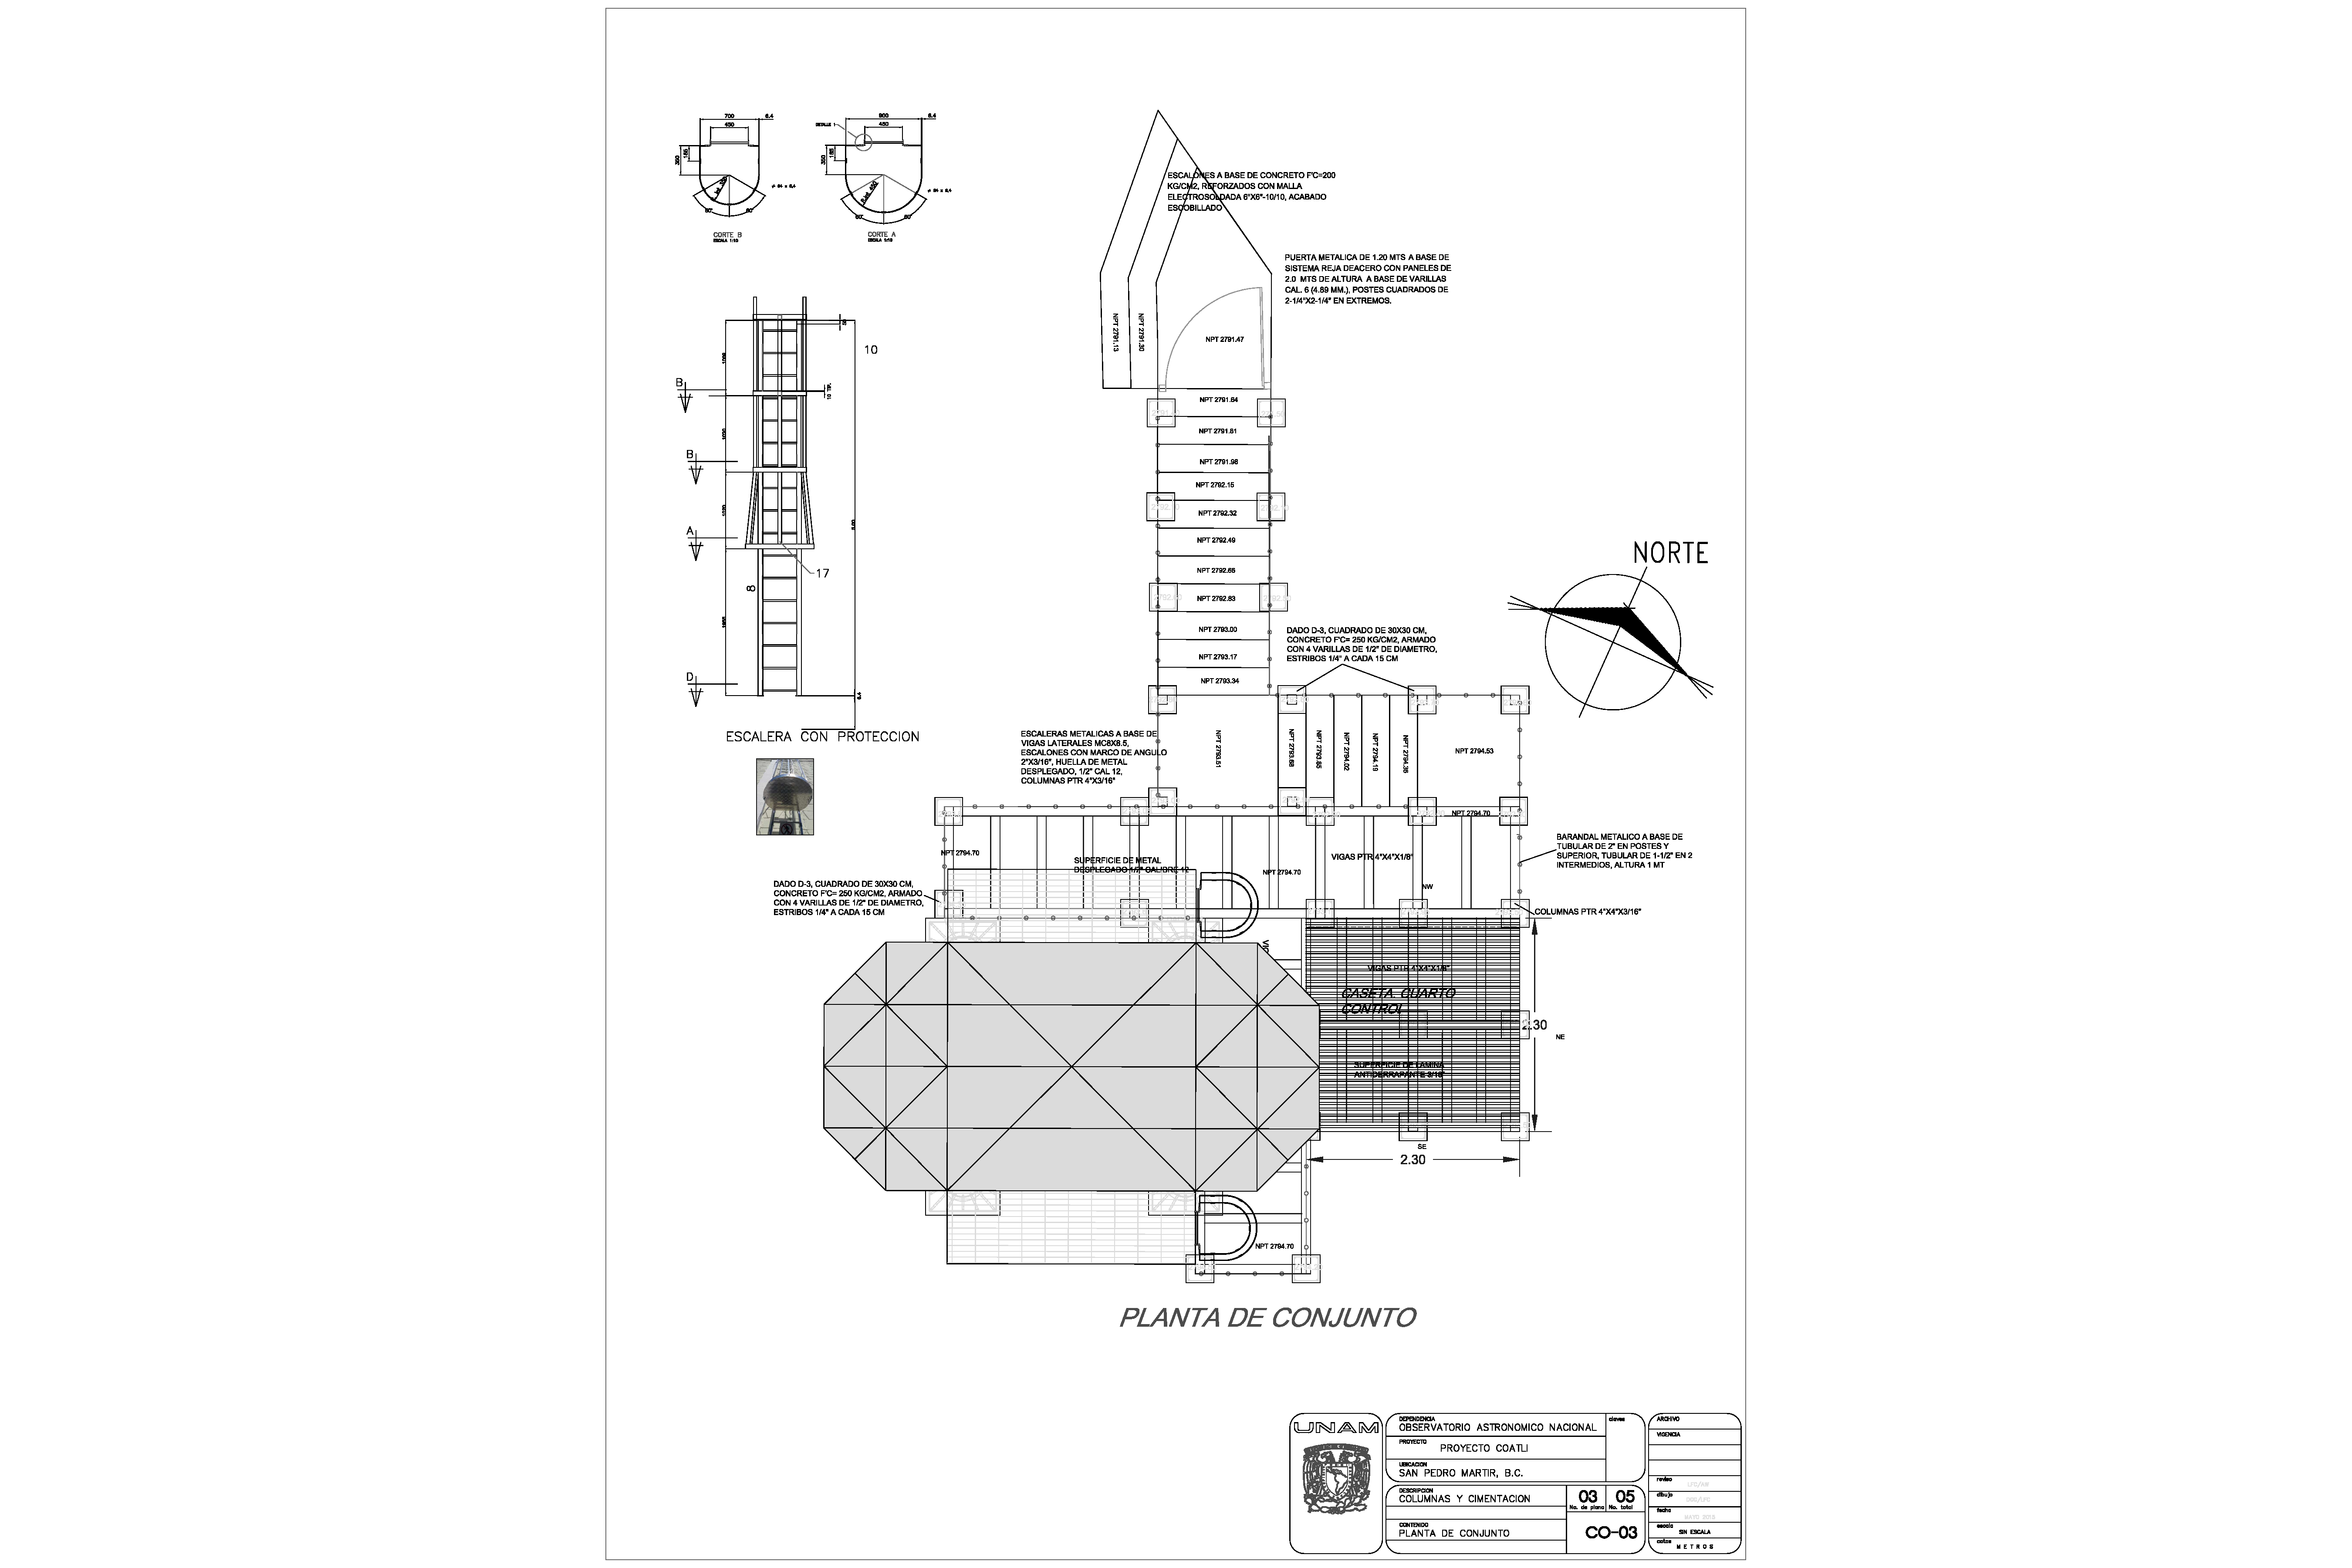
\includegraphics[width=0.95\linewidth]{figures/buildings-coatli-drawing-2015-3.pdf}
\end{center}
\caption{{\projectname} original 2015 design drawing (3 of 5).}
\label{figure:buildings-drawing-2015-3}
\end{figure*}

\begin{figure*}
\begin{center}
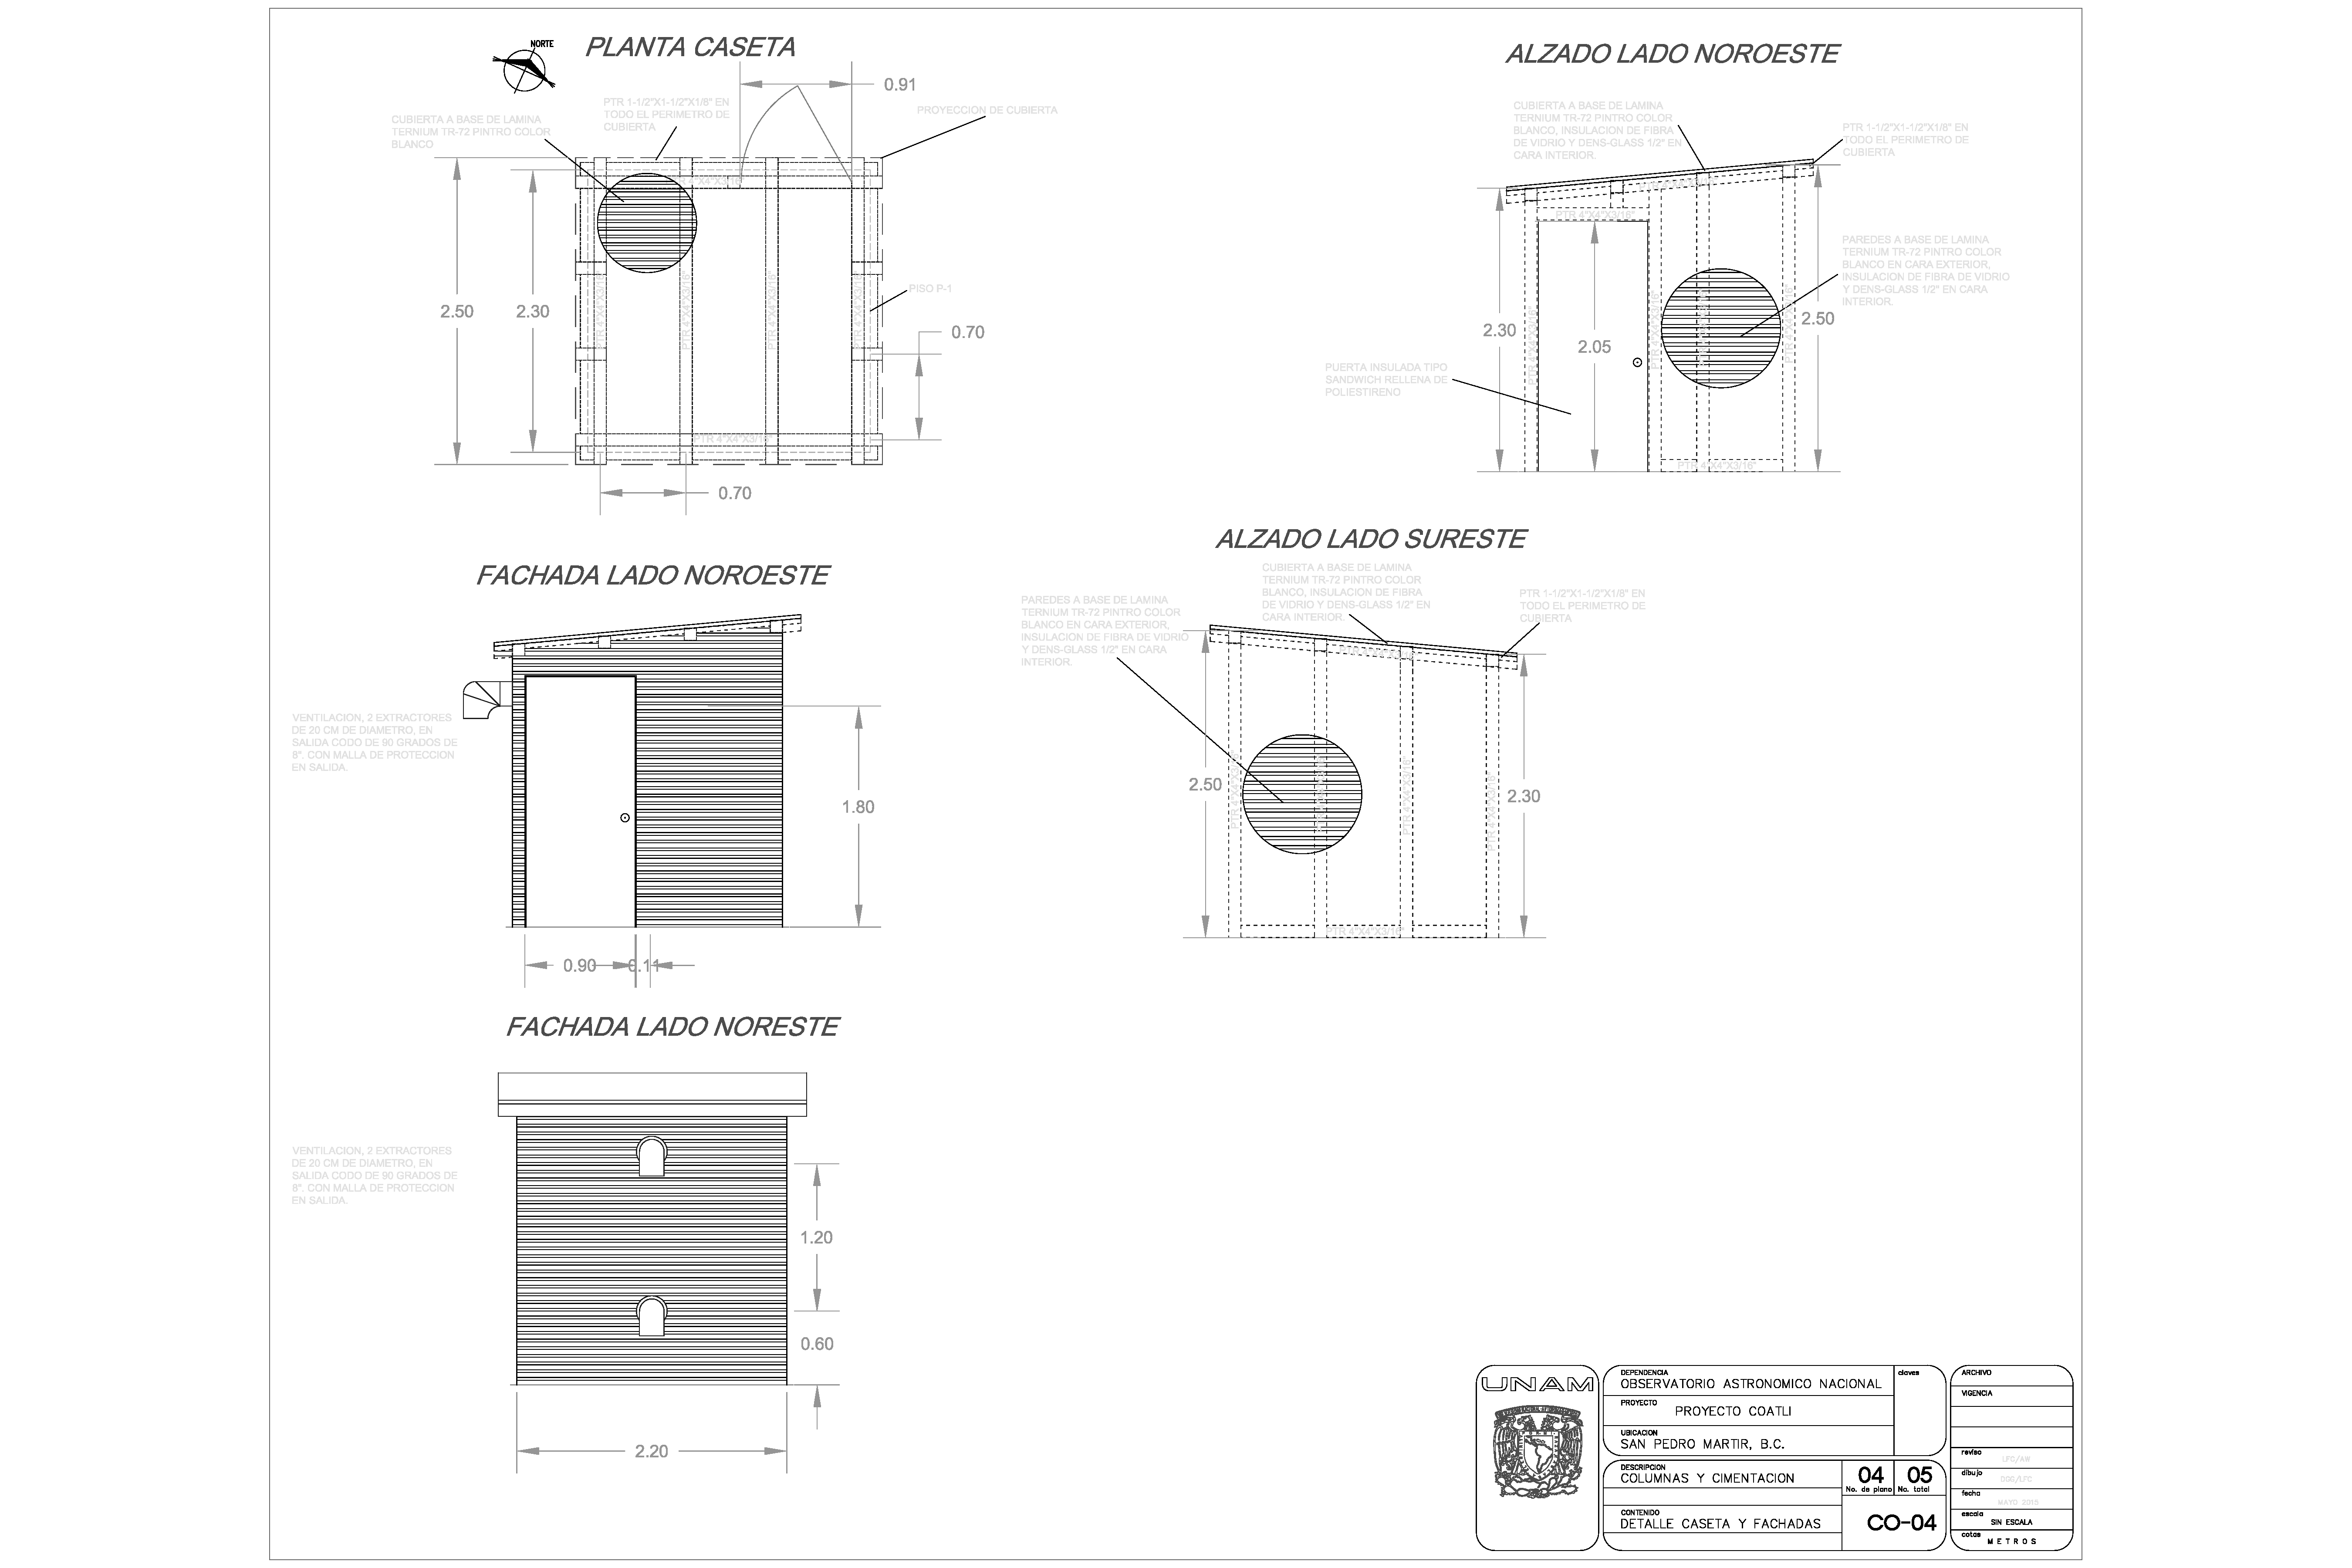
\includegraphics[height=0.95\linewidth,angle=90]{figures/buildings-coatli-drawing-2015-4.pdf}
\end{center}
\caption{{\projectname} original 2015 design drawing (4 of 5).}
\label{figure:buildings-drawing-2015-4}
\end{figure*}

\begin{figure*}
\begin{center}
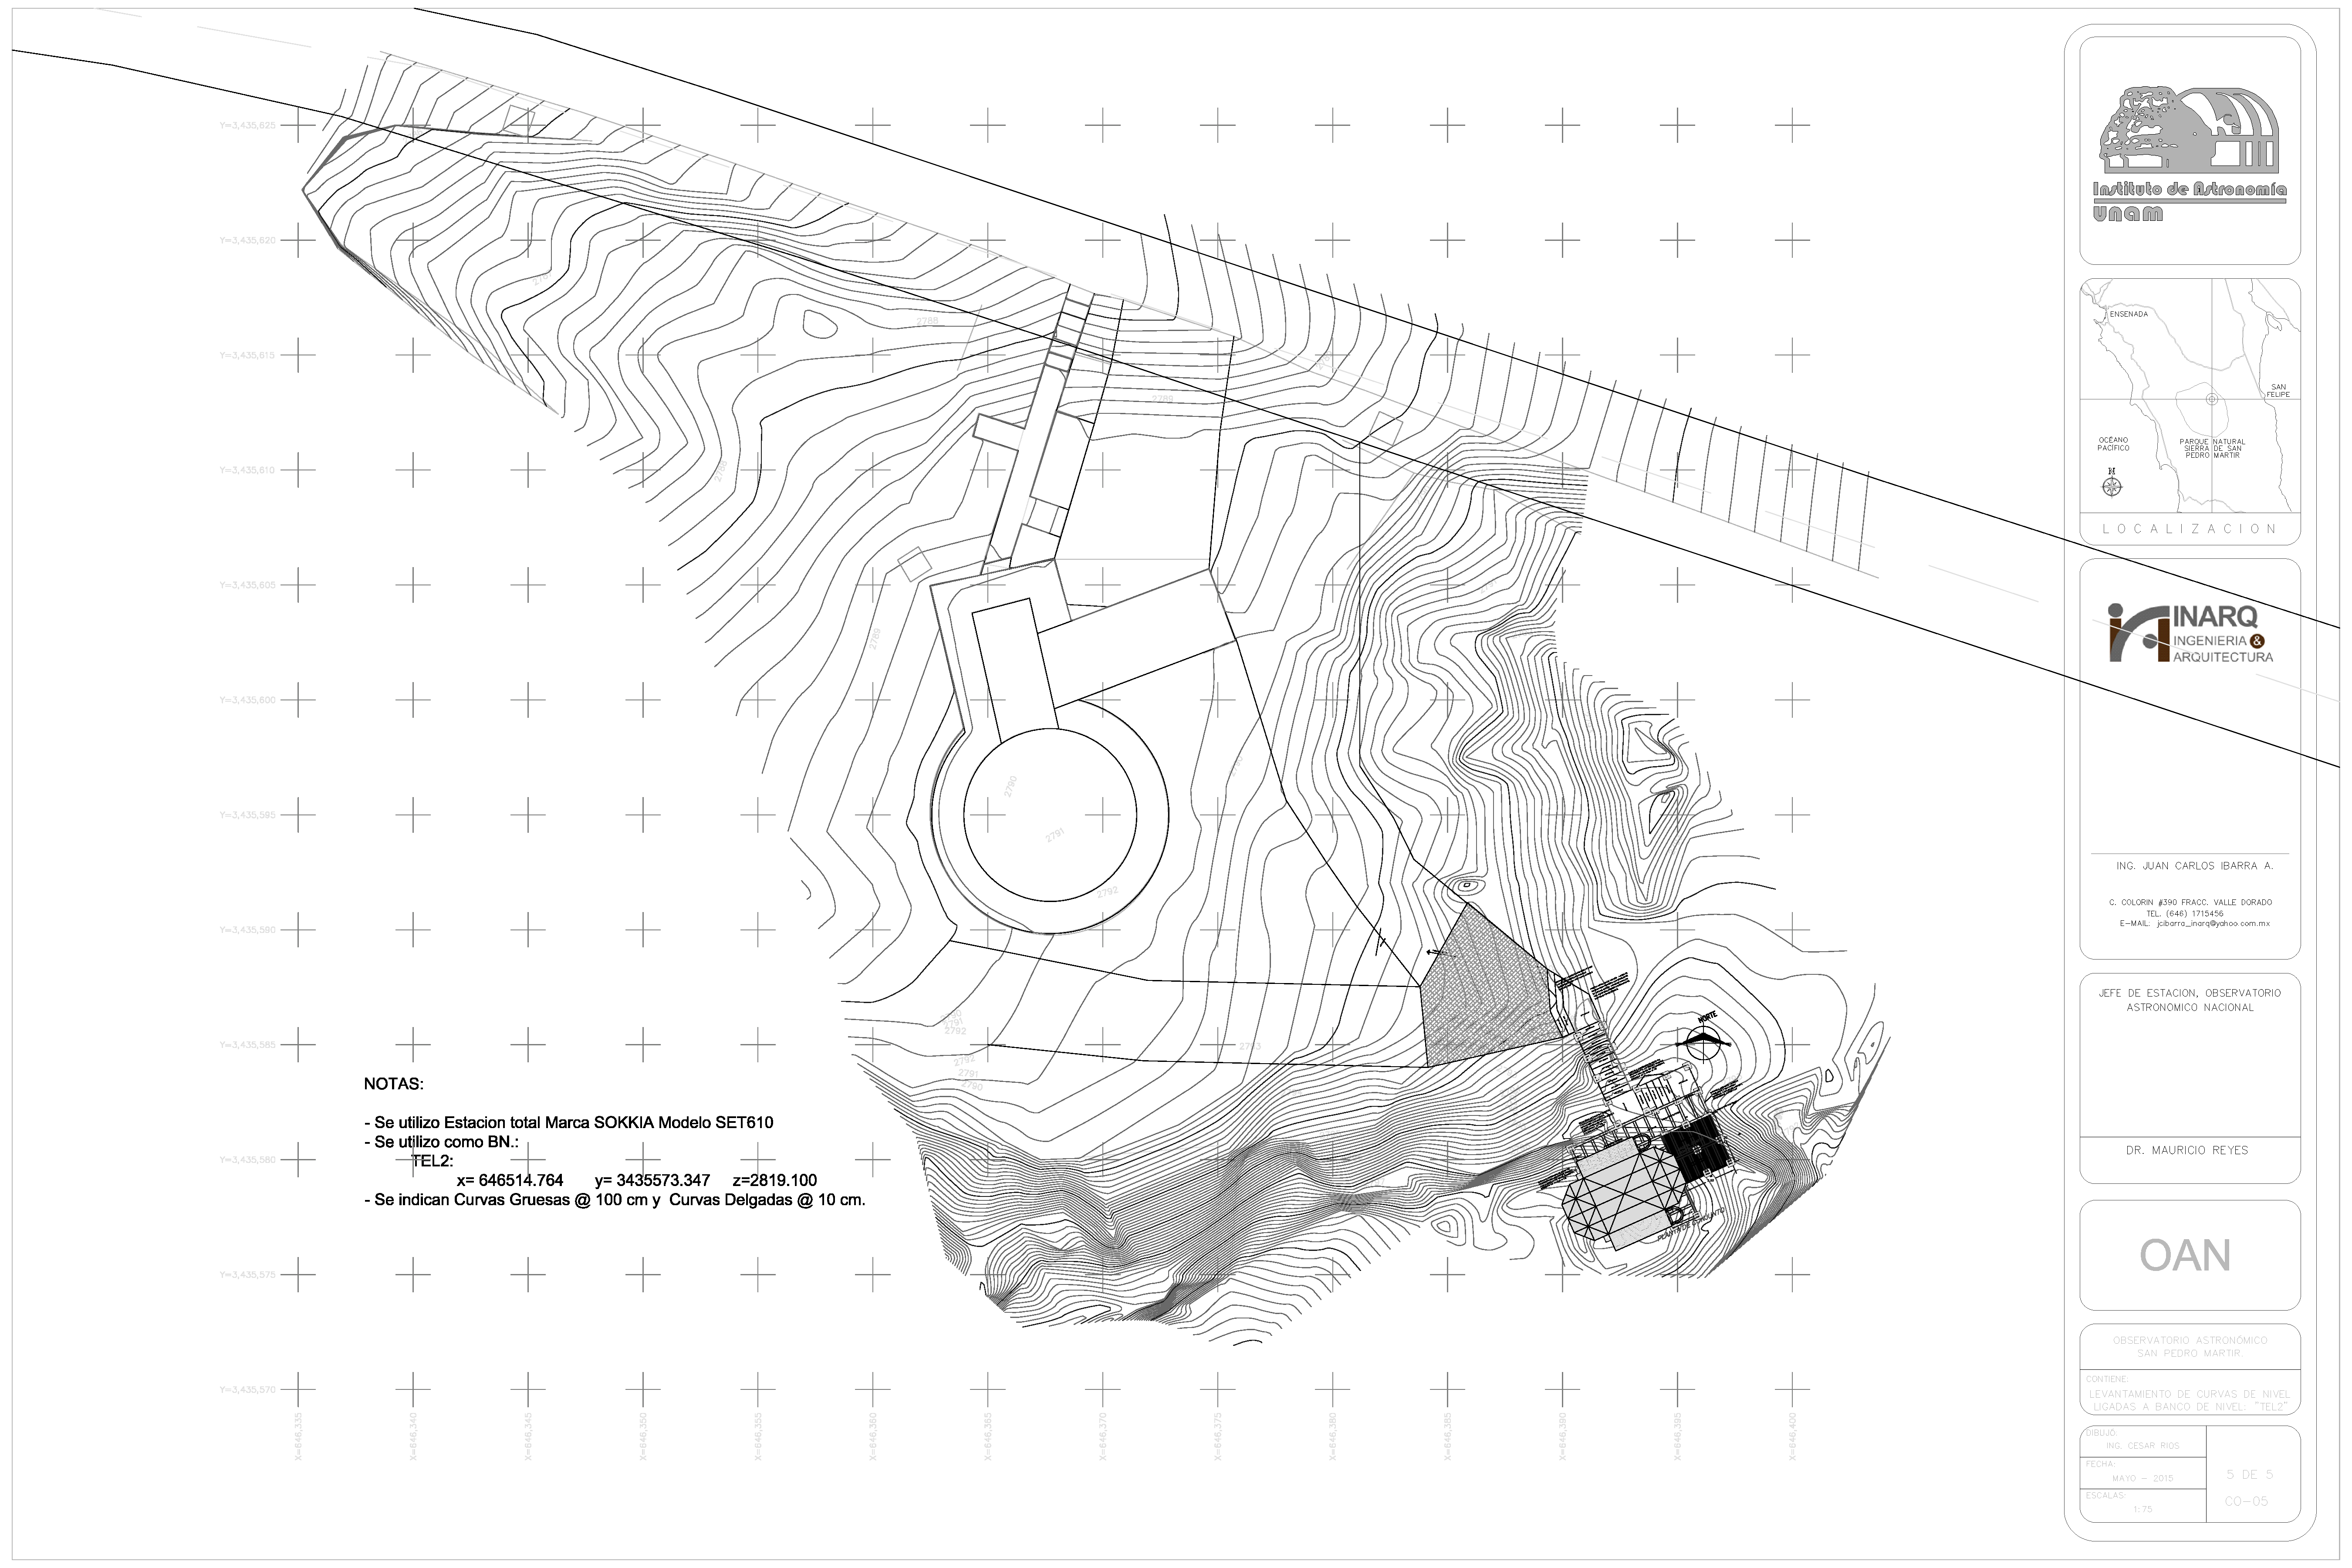
\includegraphics[height=0.95\linewidth,angle=90]{figures/buildings-coatli-drawing-2015-5.pdf}
\end{center}
\caption{{\projectname} original 2018 design drawing (5 of 5).}
\label{figure:buildings-drawing-2015-5}
\end{figure*}

\begin{figure*}
\begin{center}
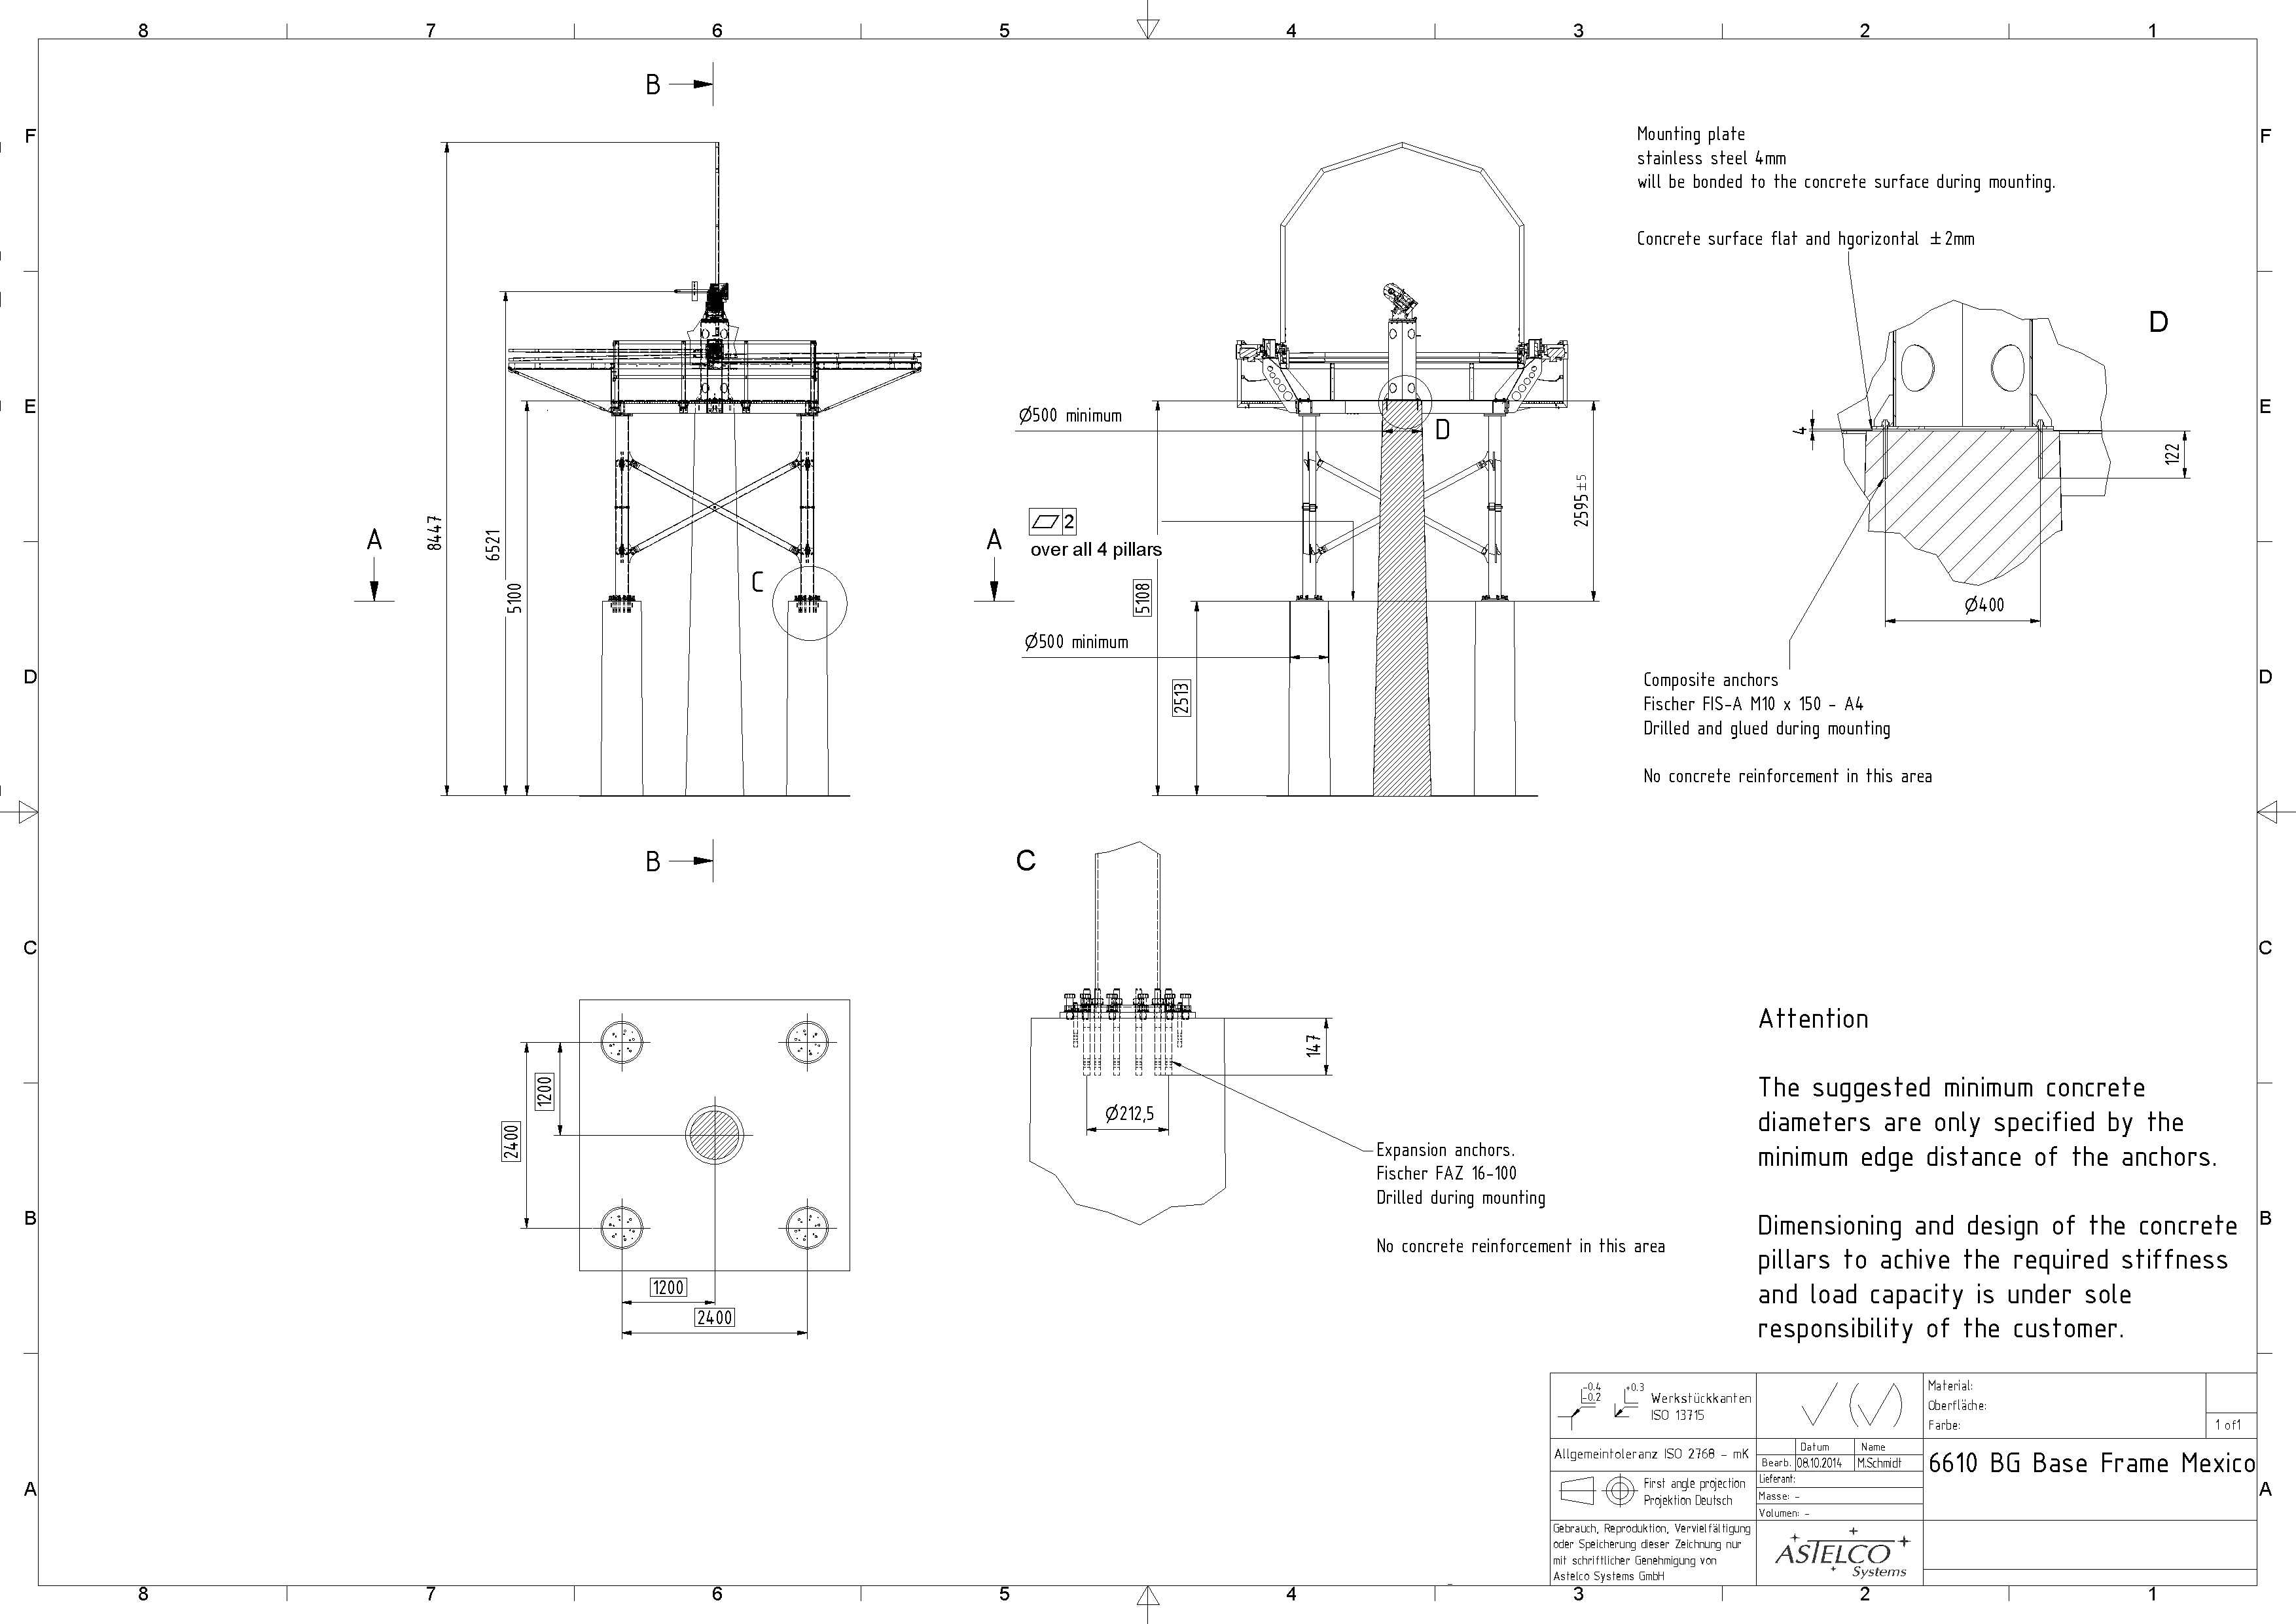
\includegraphics[height=0.95\linewidth,angle=90]{figures/buildings-coatli-astelco-enclosure-drawing-6610}
\end{center}
\caption{{\projectname} ASTELCO Platform and Telescope Pillar.}
\label{figure:buildings-drawing-astelco}
\end{figure*}

\begin{figure*}
\begin{center}
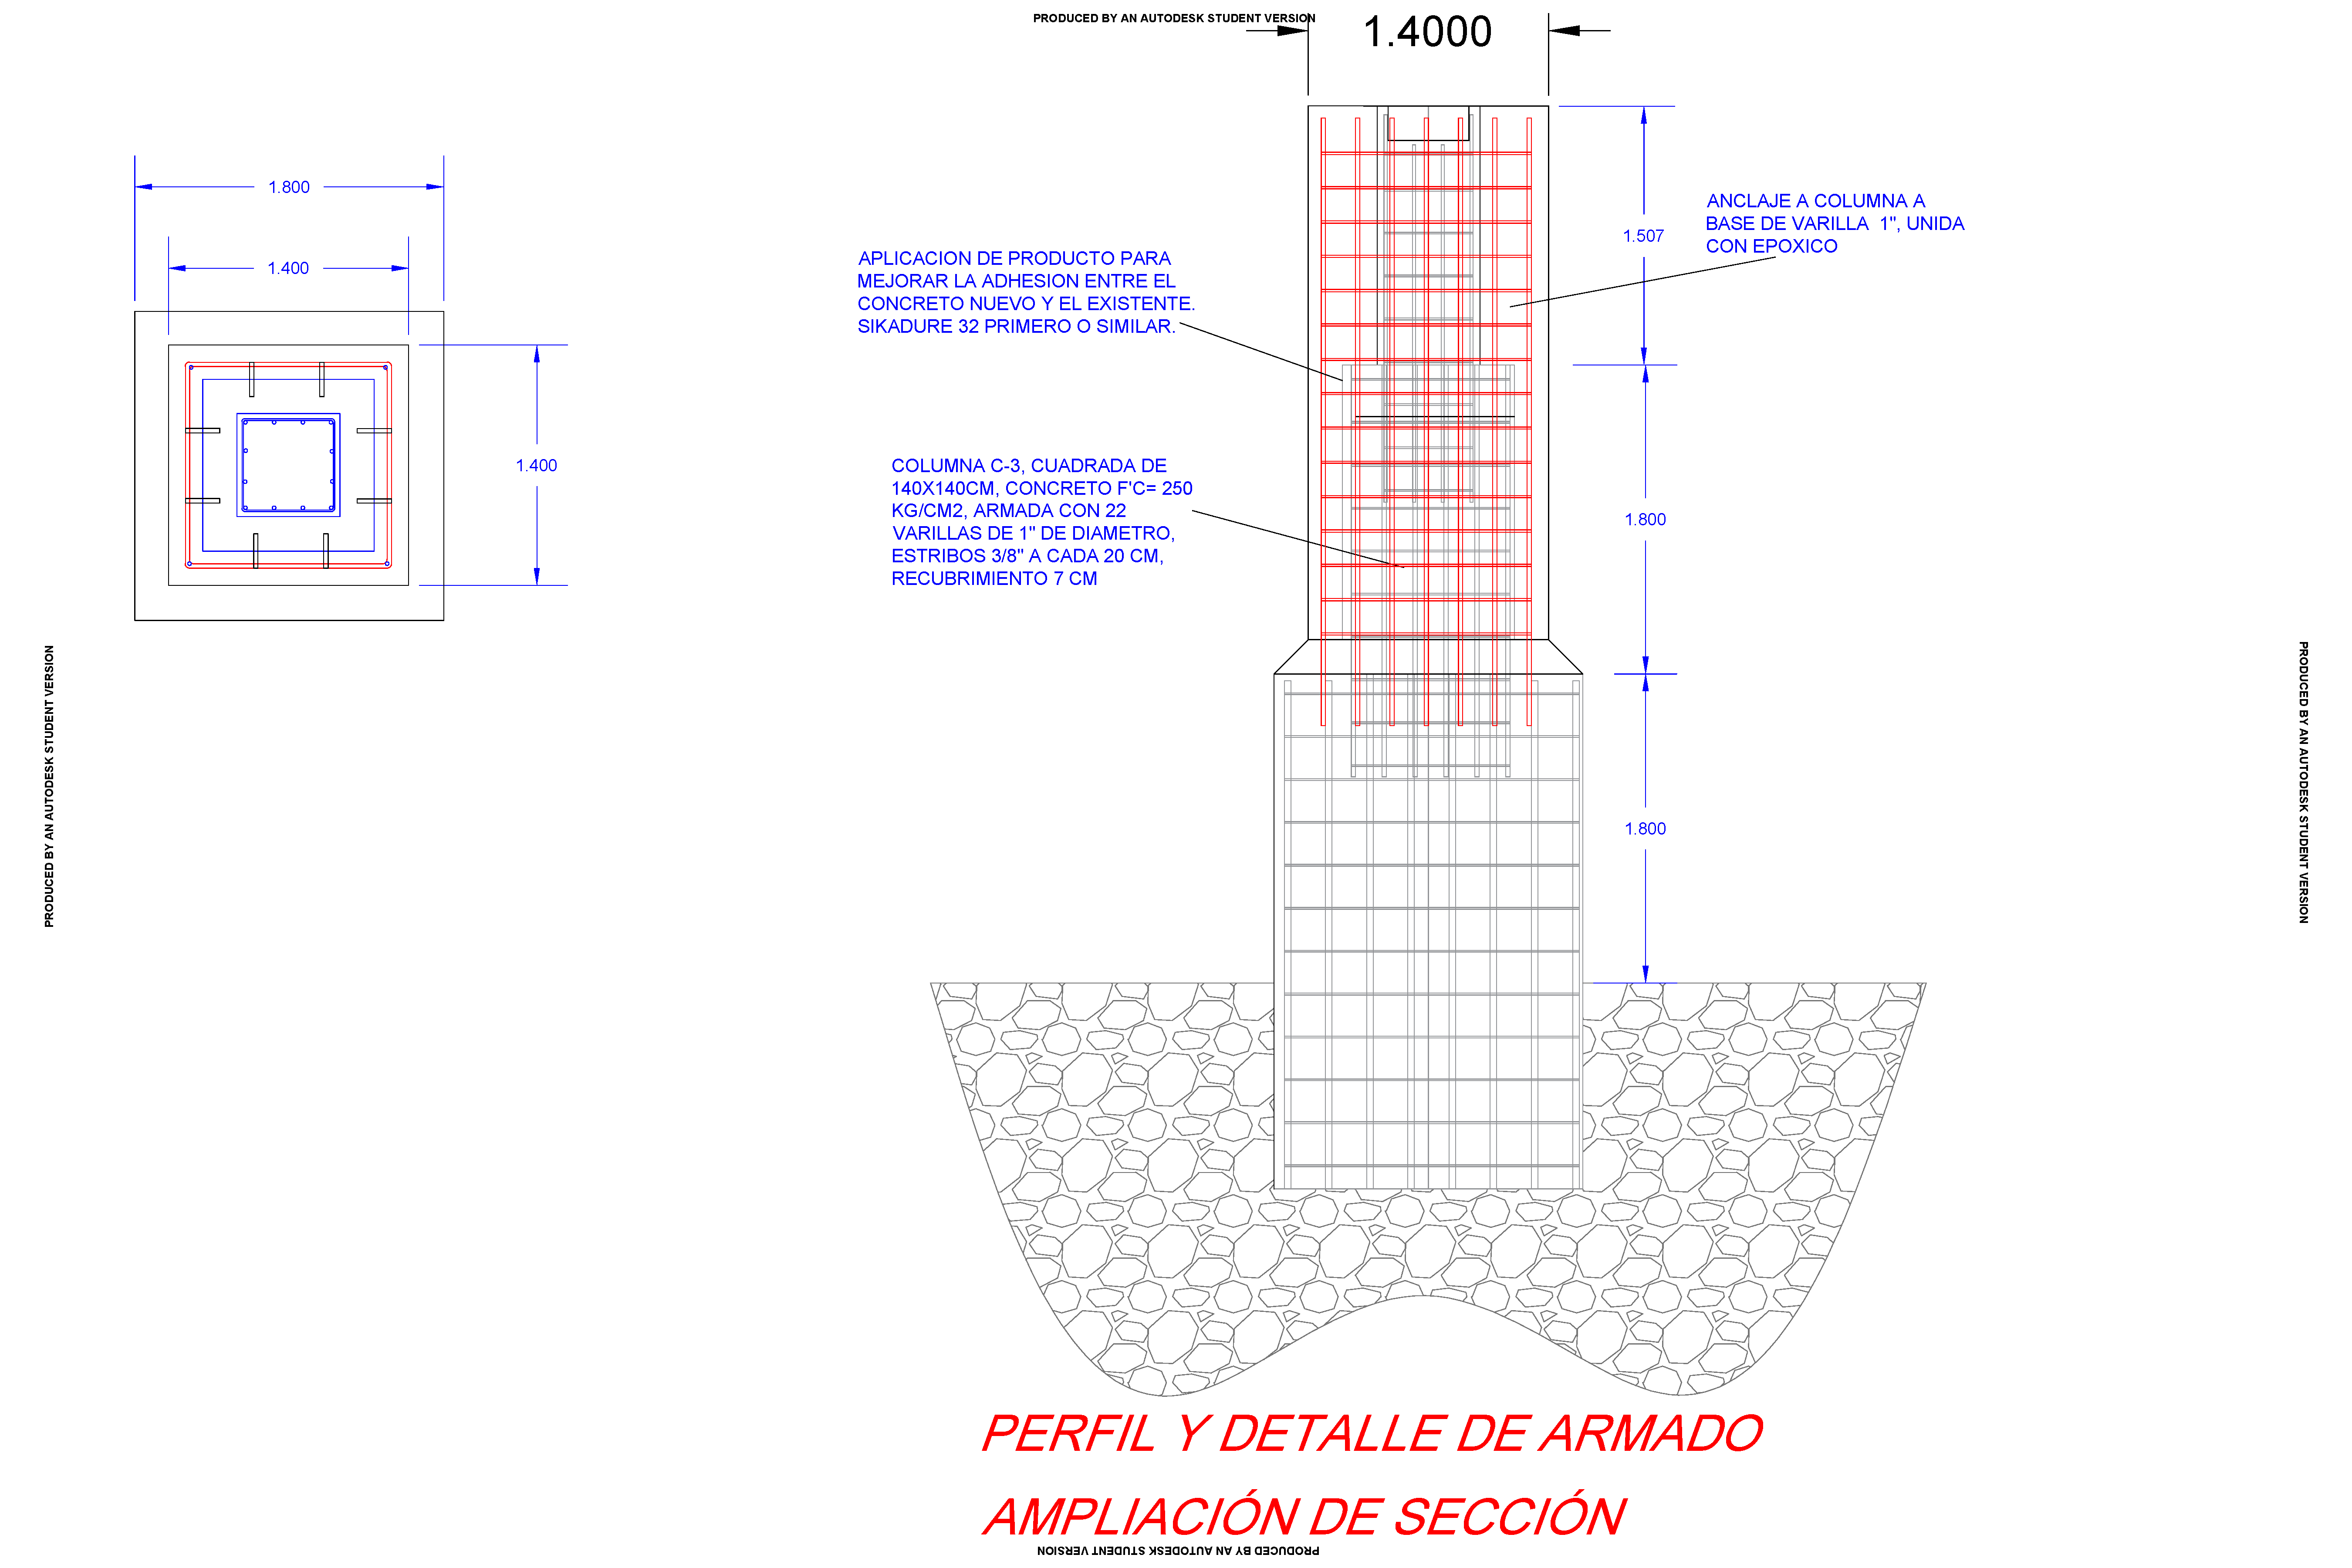
\includegraphics[height=0.95\linewidth,angle=90]{figures/buildings-coatli-drawing-2018-1.pdf}
\end{center}
\caption{{\projectname} Modified 2018 design drawing (1 of 3).}
\label{figure:buildings-drawing-2018-1}
\end{figure*}

\begin{figure*}
\begin{center}
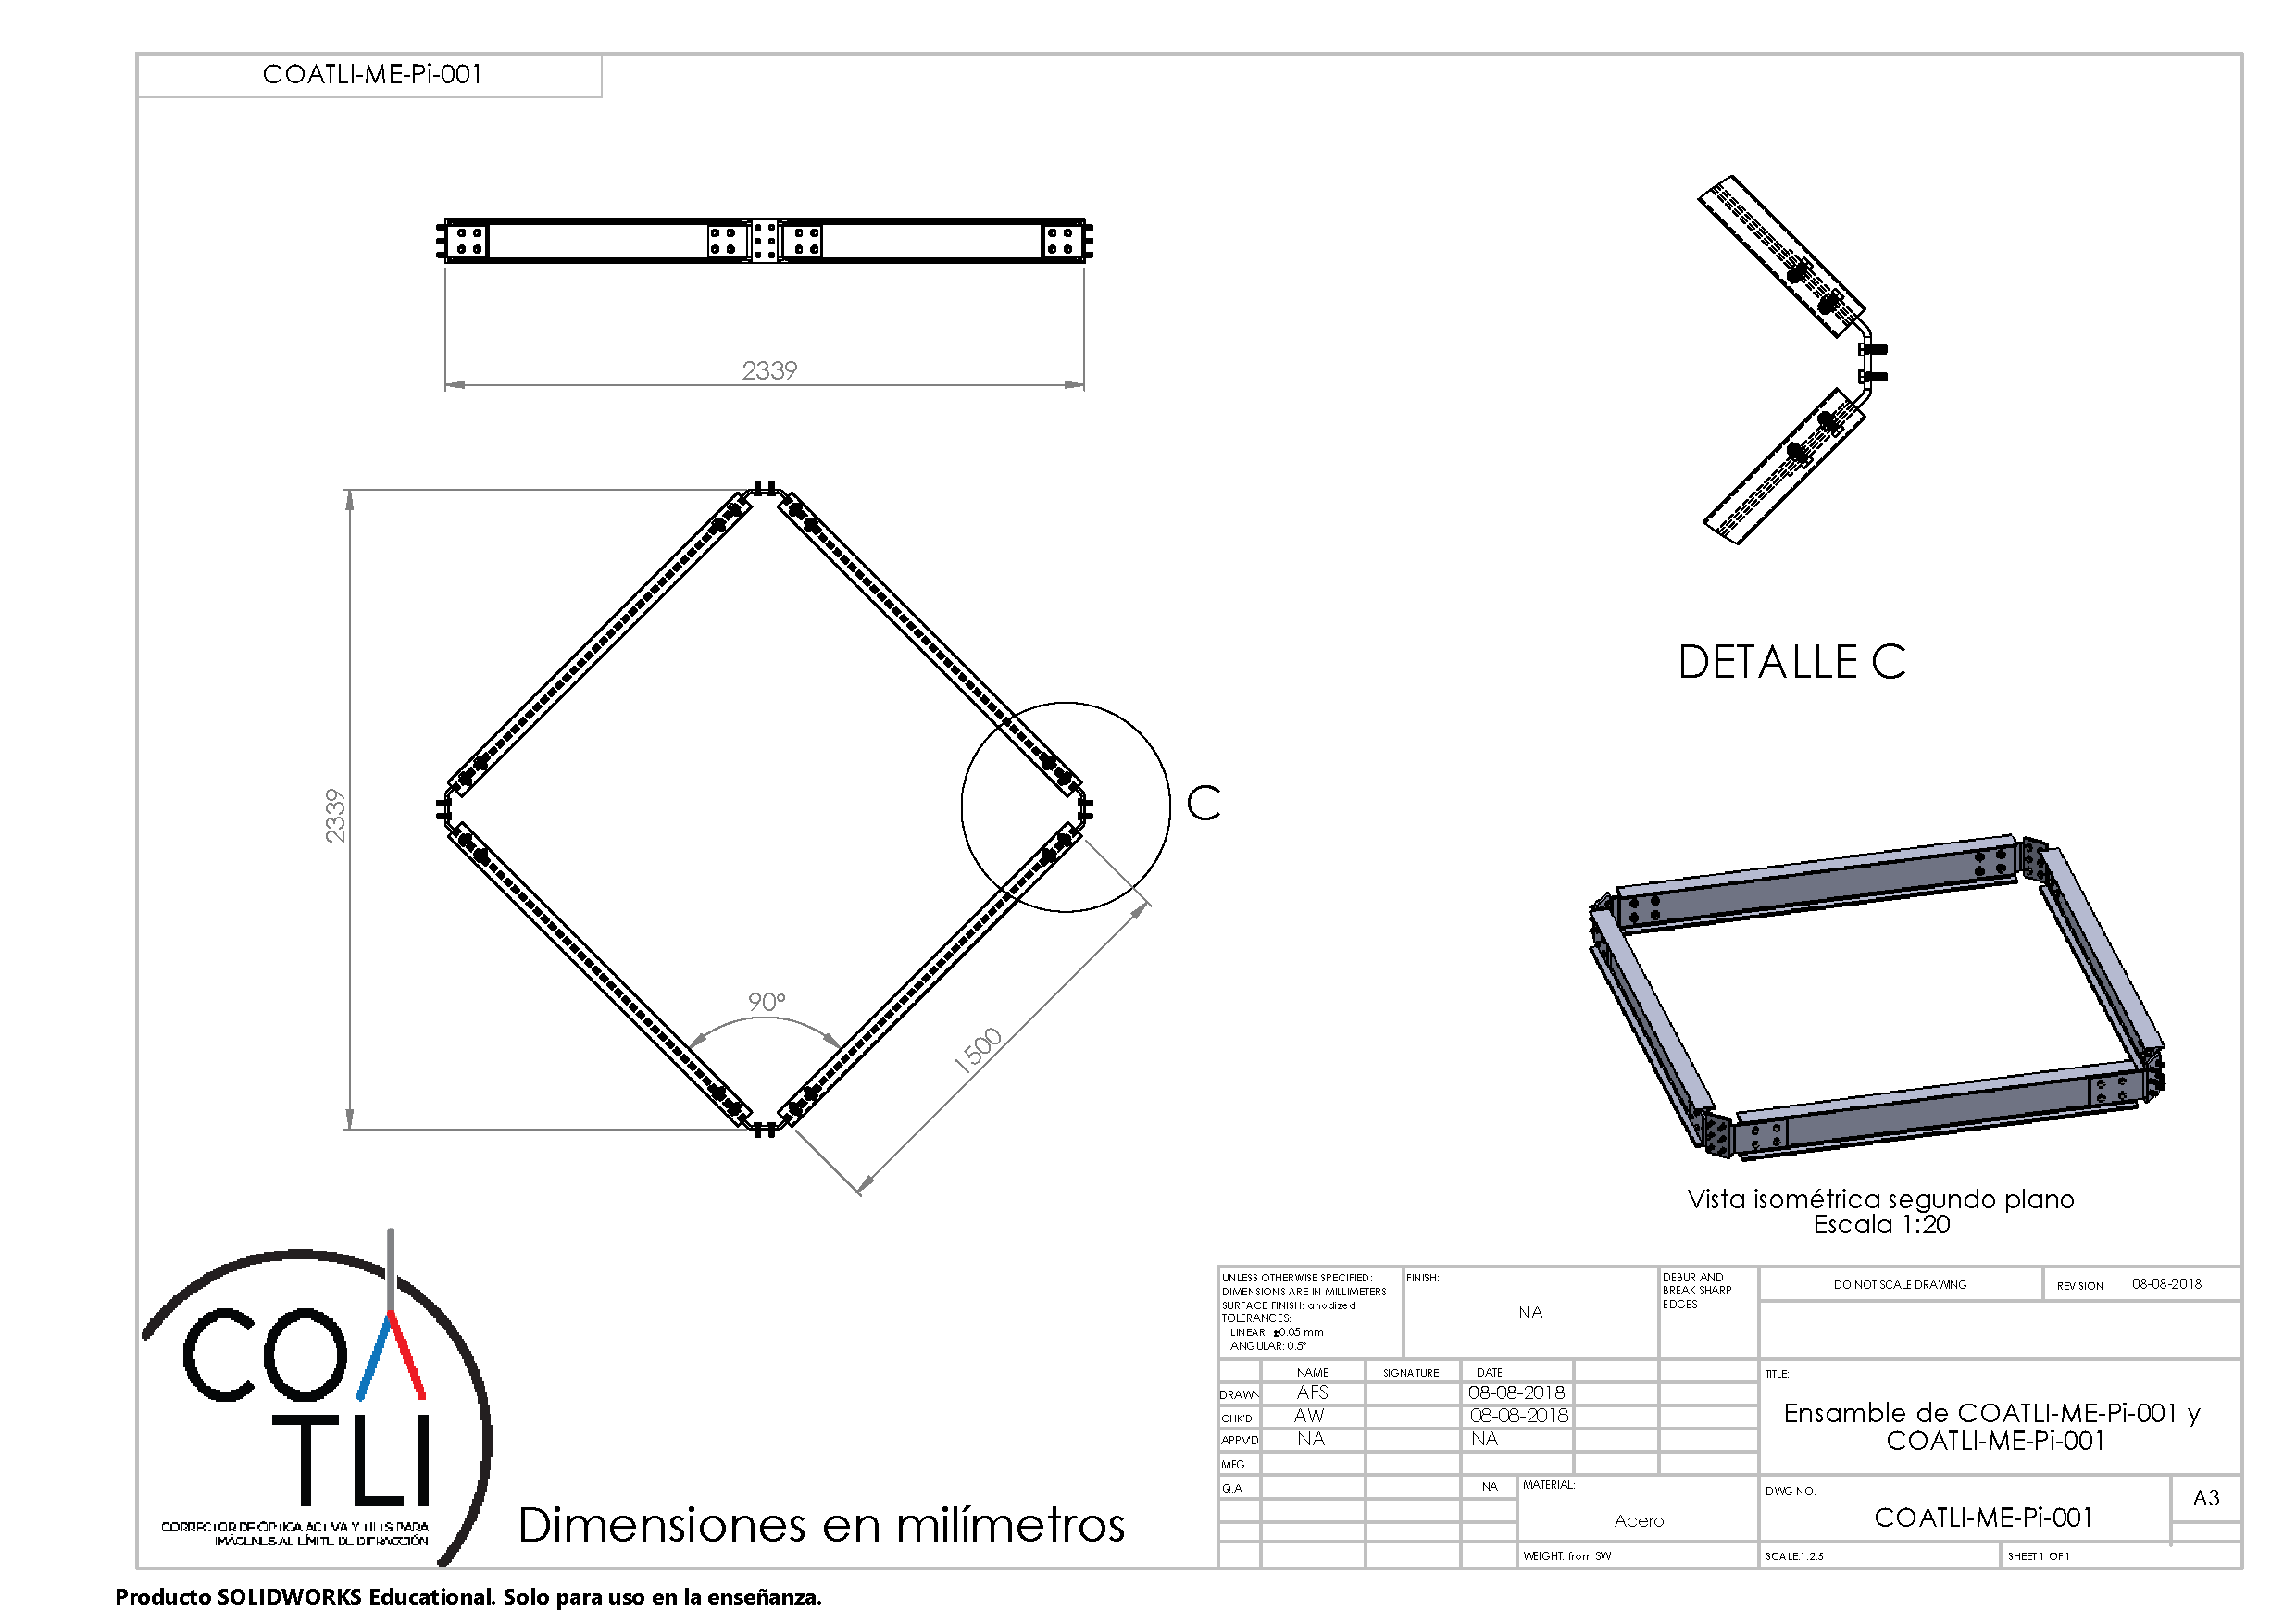
\includegraphics[height=0.95\linewidth,angle=90]{figures/buildings-coatli-drawing-2018-2.pdf}
\end{center}
\caption{{\projectname} Modified 2018 design drawing (2 of 3).}
\label{figure:buildings-drawing-2018-2}
\end{figure*}

\begin{figure*}
\begin{center}
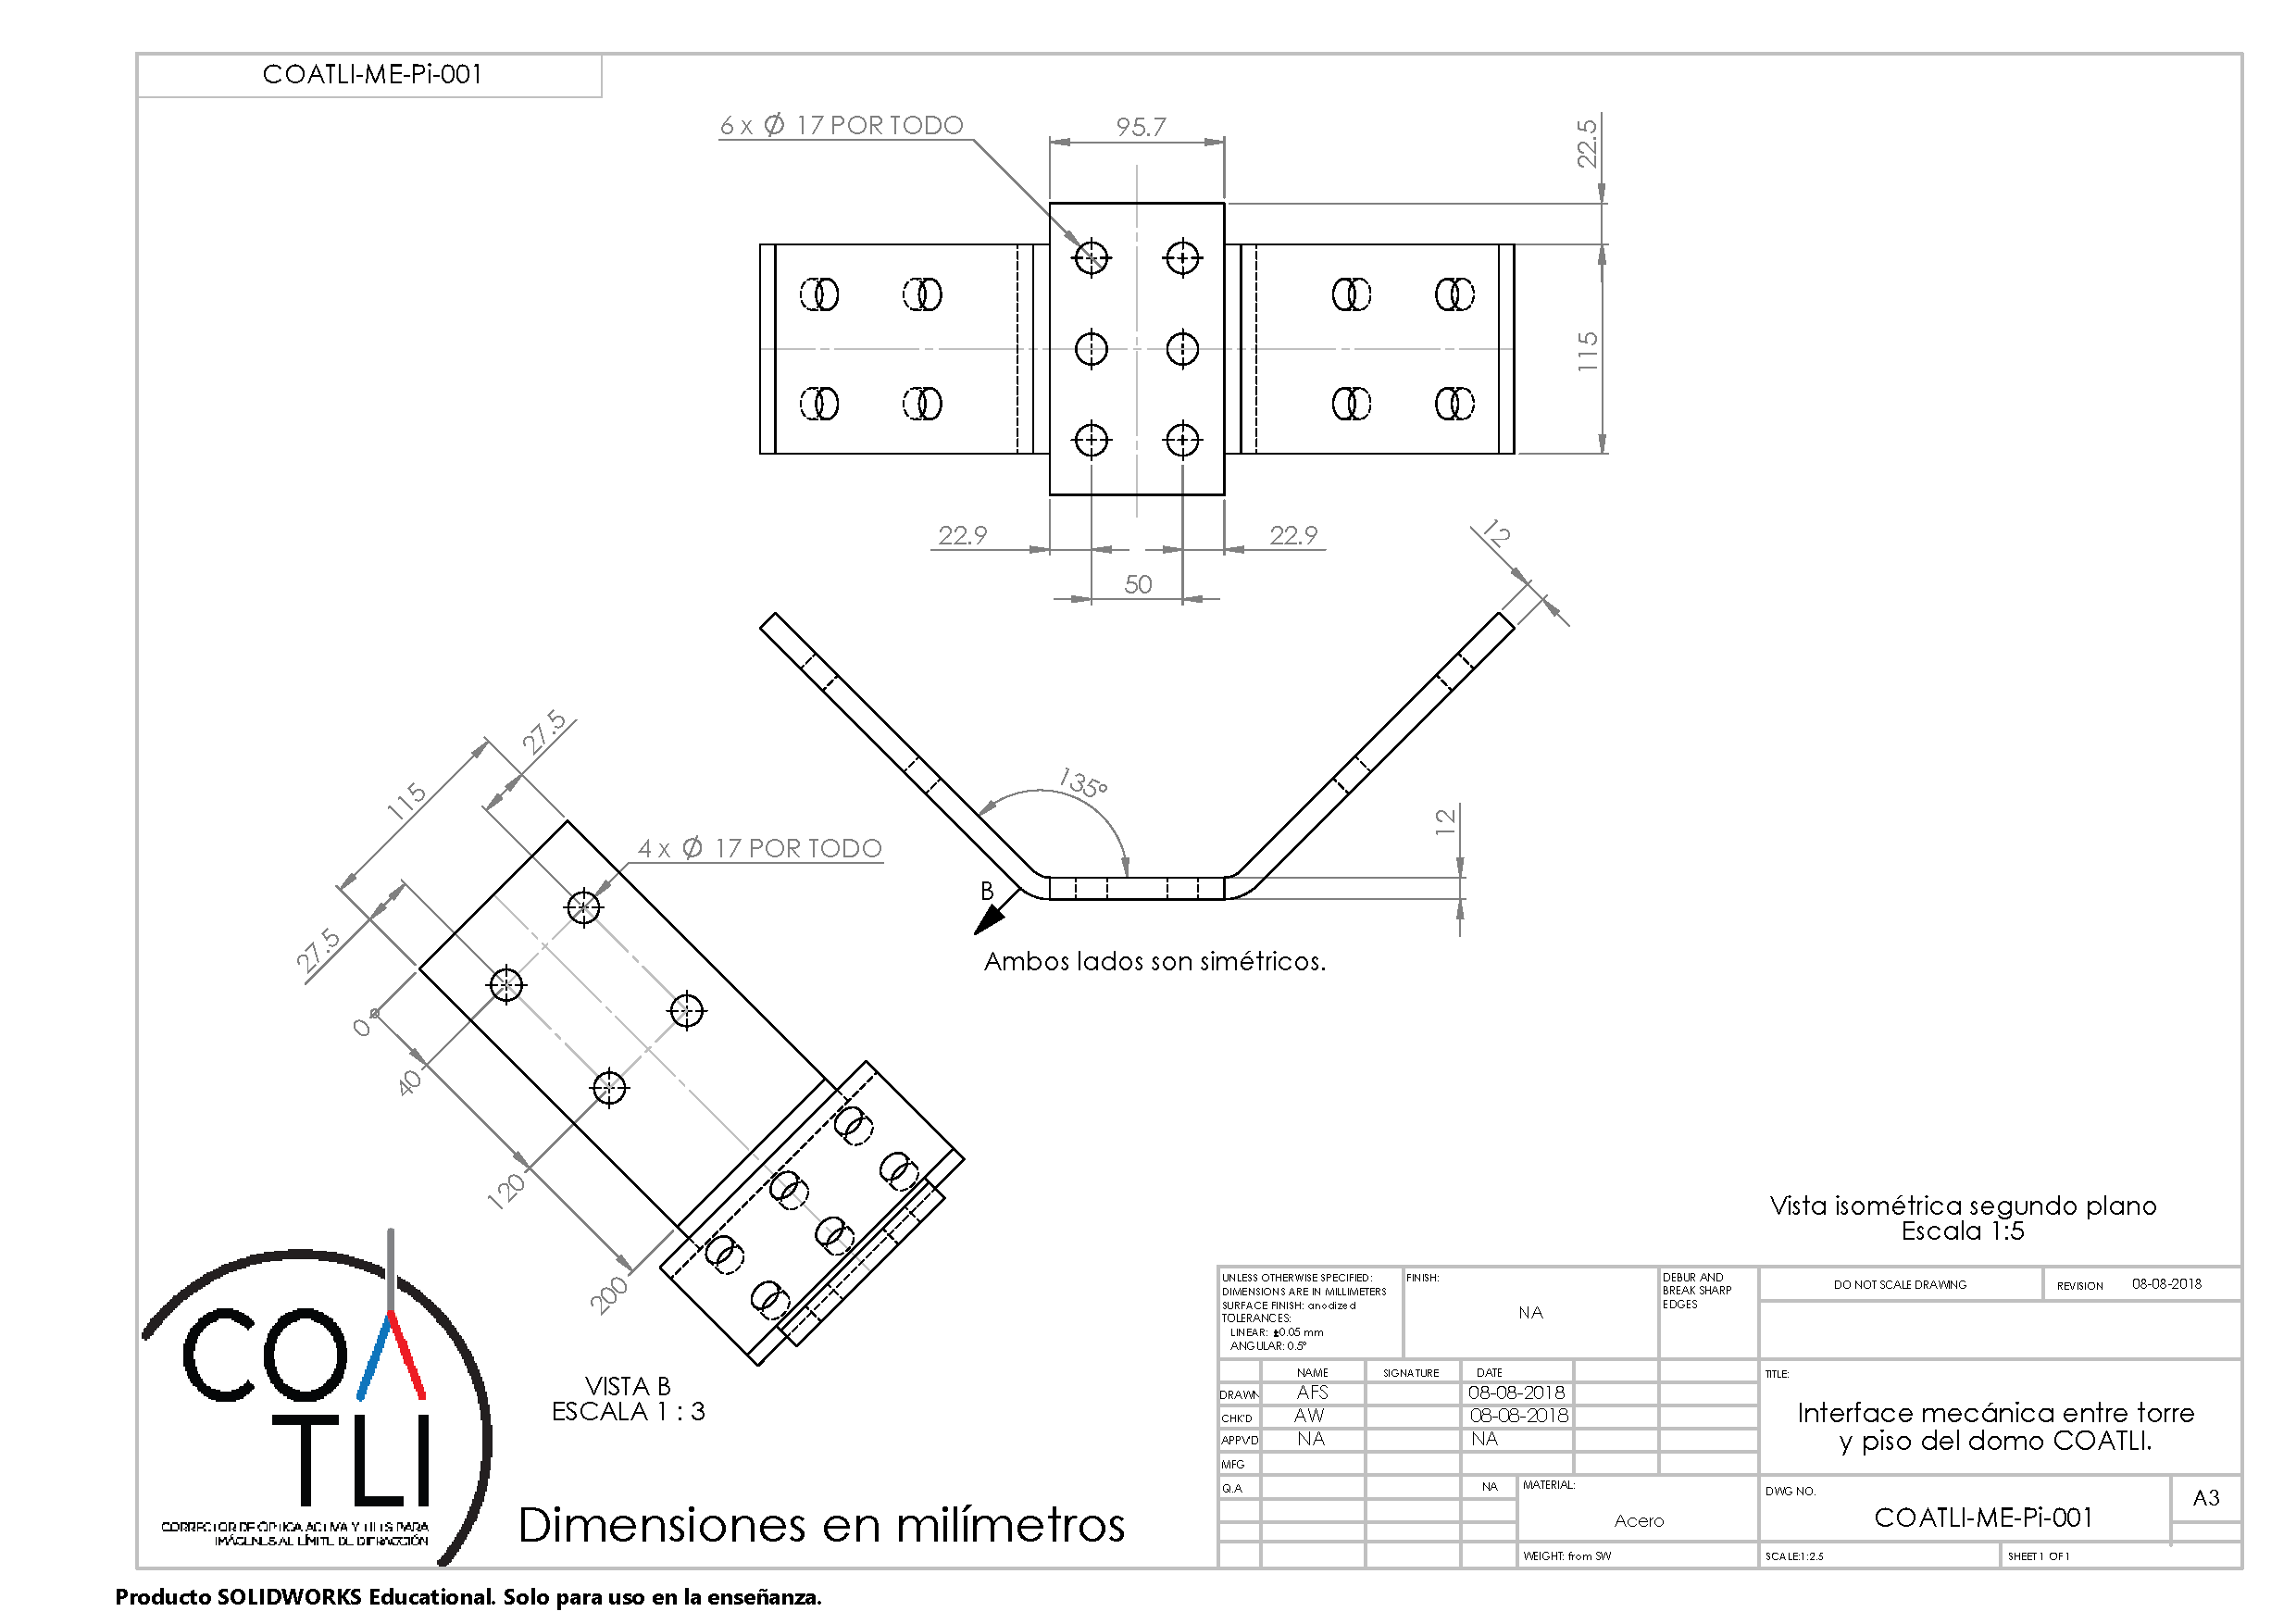
\includegraphics[height=0.95\linewidth,angle=90]{figures/buildings-coatli-drawing-2018-3.pdf}
\end{center}
\caption{{\projectname} Modified 2018 design drawing (3 of 3).}
\label{figure:buildings-drawing-2018-3}
\end{figure*}
\fi

\ifddotioan

The shed, access, and tower are constructed on open space to the north of the 84-cm building. The buildings and structures were constructed in 2016 and the enclosure installed in 2017.

Figures~\ref{figure:buildings-drawing-2016-1} to \ref{figure:buildings-drawing-2016-3} show the 2016 design drawings for the shed, access staircase and walkways, and the concrete columns that support the platform and telescope. The original design was largely based on that of COATLI, but with simplifications for the easier site and a slightly different telescope column. The DDOTI telescope column extended 40 cm above the platform floor (the COATLI column is flush with the platform floor) to reduce the height of the steel pier and increase its stability. Figure  \ref{figure:buildings-drawing-astelco} shows the ASTELCO ARTS platform and the ASTELCO steel pillar mounted on the concrete columns (although this drawing is for COATLI, the DDOTI enclosure is identical except for the perforation in the platform floor). Figure  \ref{figure:buildings-drawing-astelco-pier} shows the ASTELCO pier. The center of rotation of the mount axes is about 6.5 meters above the ground level.

During the summer of 2016, the design of the telescope column was changed without this change being adequately communicated to the project. The telescope concrete column  originally was designed with three parts, each square in cross section and tapering from 1.8, 1.2, and 0.6 meters to a side, like the COATLI column. The design was changed so that the middle and upper sections were uniformly 1.0 meters to a side (although some erroneous vestiges of the original column remain in Figures~\ref{figure:buildings-drawing-2016-1}). Fortunately, this change was caught in time to allow the platform to be modified.

The original design was intended to be oriented with the long-axis of the enclosure aligned with geographic N-S (see Figure~\ref{figure:buildings-drawing-2016-2}). However, when the site was laid out, the surveyor made a sign error in the magnetic deviation. Instead of being aligned with geographic north (11 degrees west of magnetic north) the structures were aligned 22 degrees east of geographic north (11 degrees east of magnetic north). This error was not detected until the lower part of the telescope column had been poured. Fortunately, the column and enclosure could still accommodate the pier, mount, and telescopes.

\begin{figure*}
\begin{center}
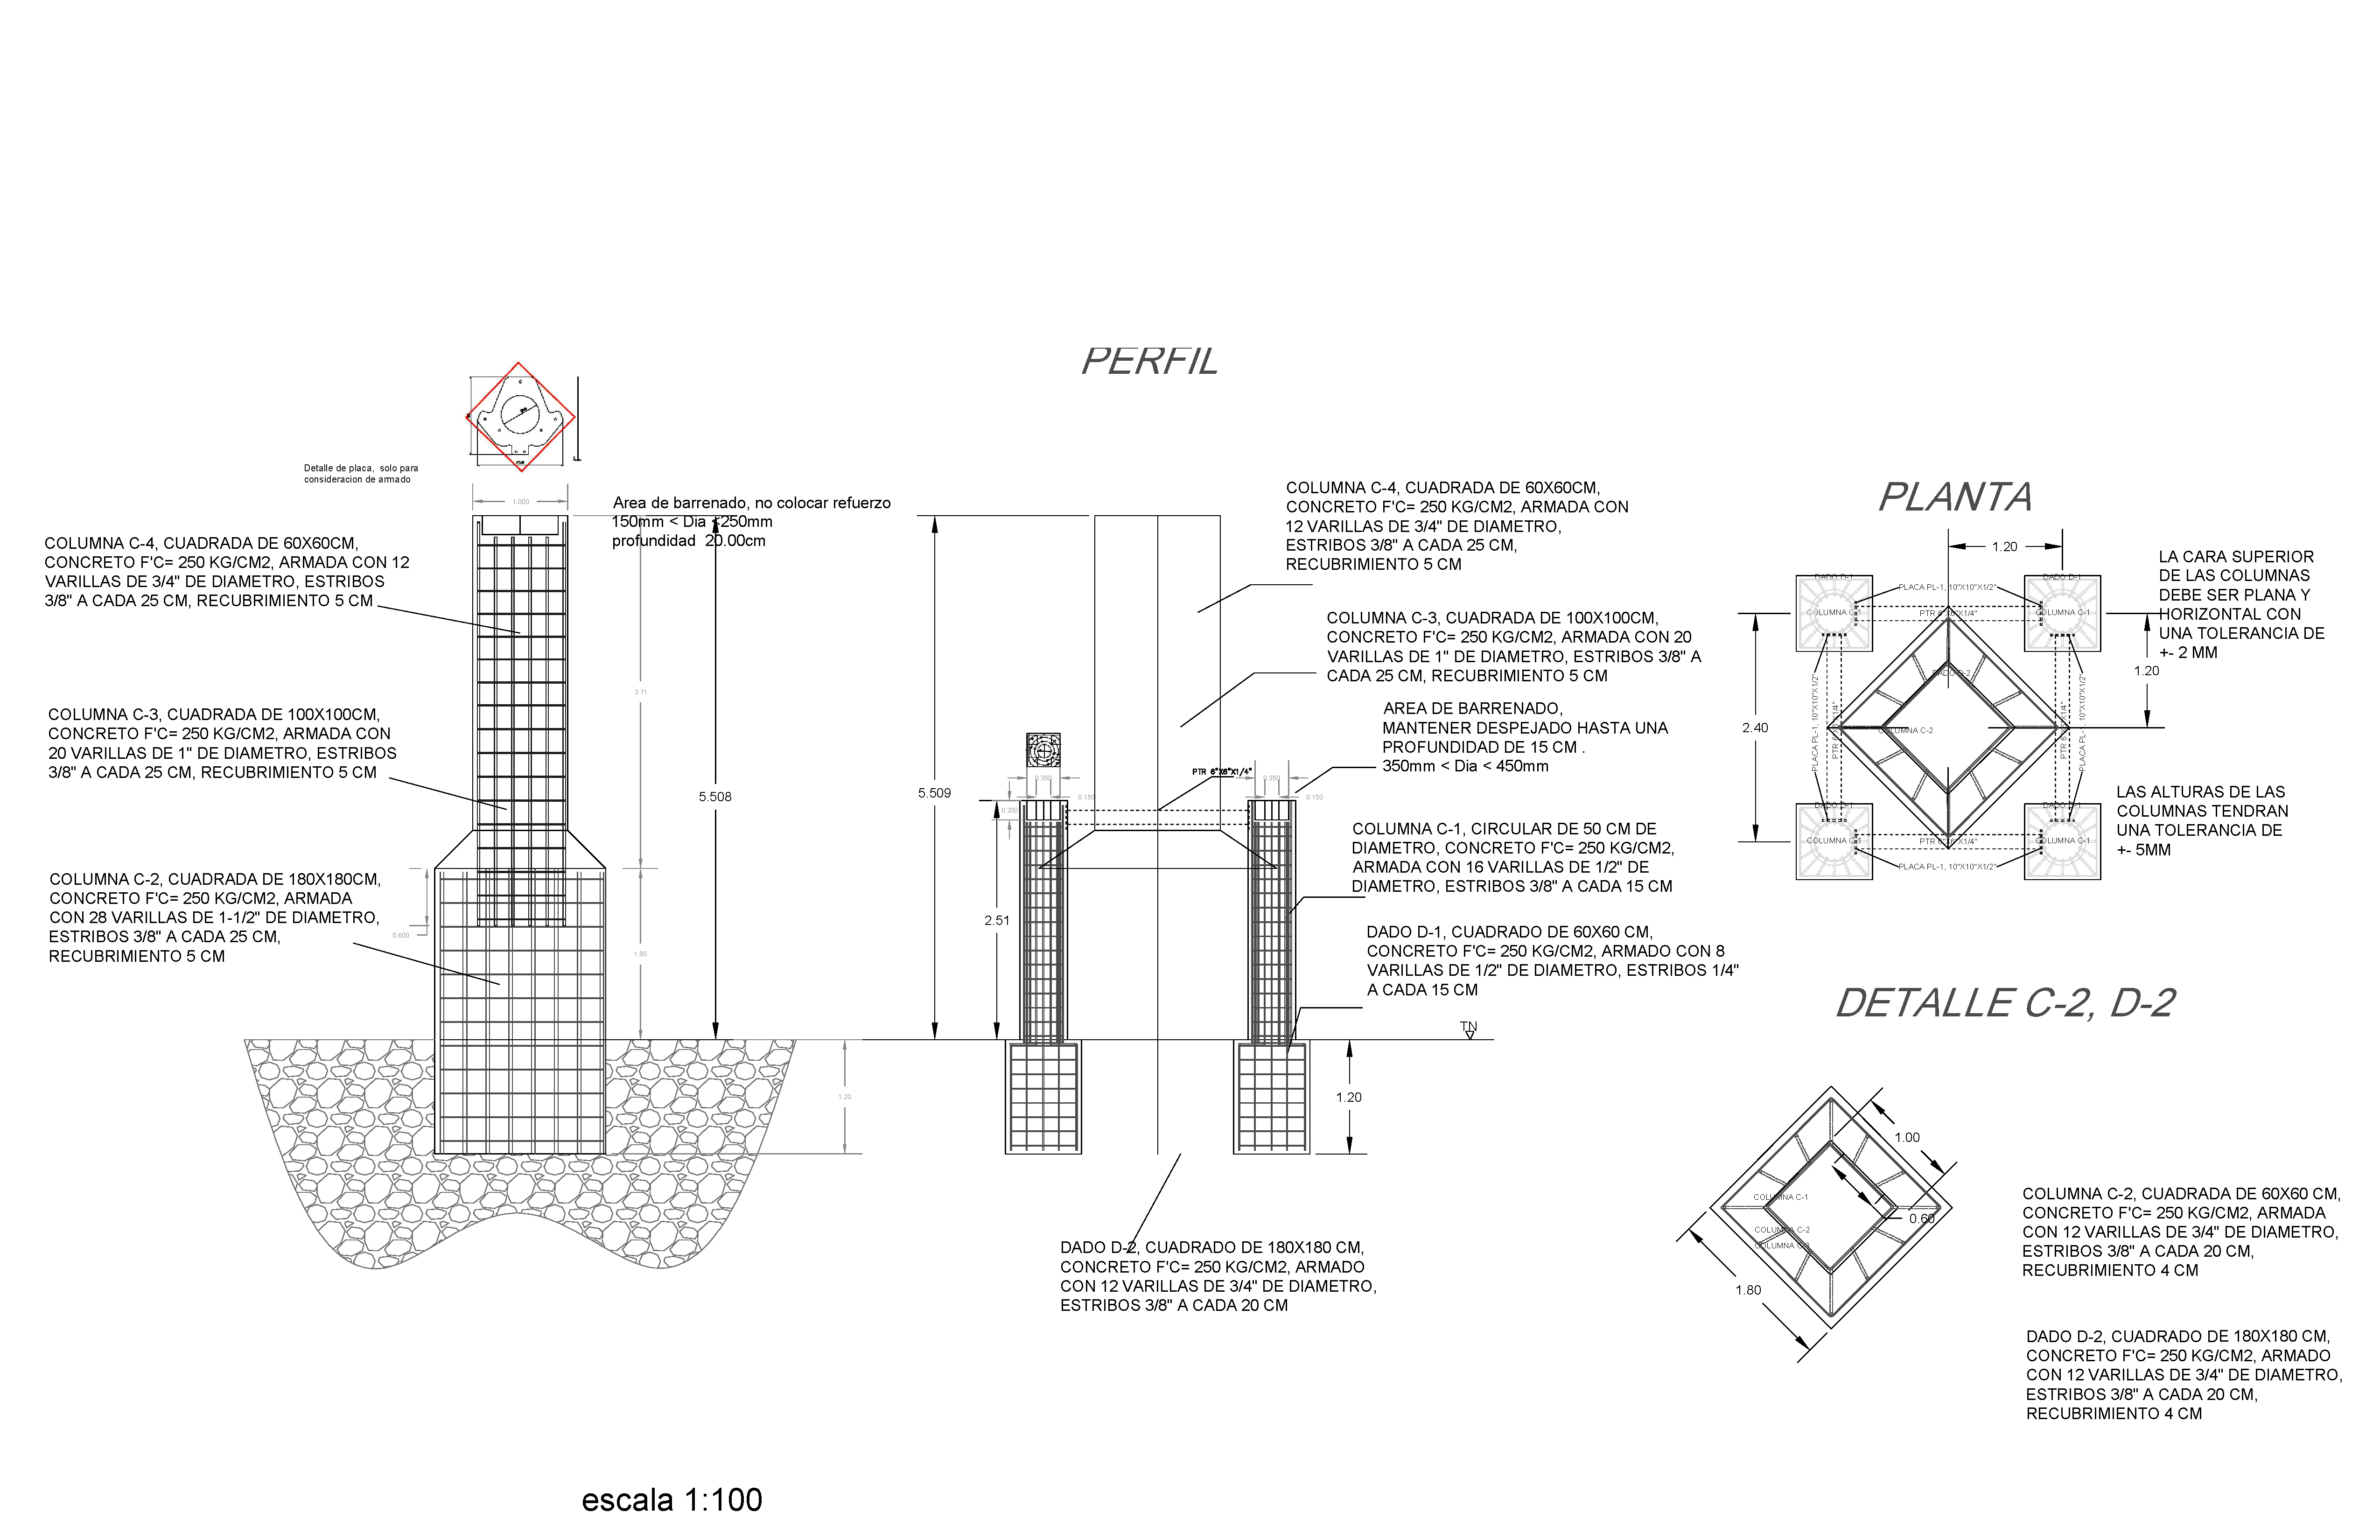
\includegraphics[height=0.95\linewidth,angle=90]{figures/buildings-ddoti-drawing-2016-1.pdf}
\end{center}
\caption{{\projectname} original 2016 design drawing (1 of 3).}
\label{figure:buildings-drawing-2016-1}
\end{figure*}

\begin{figure*}
\begin{center}
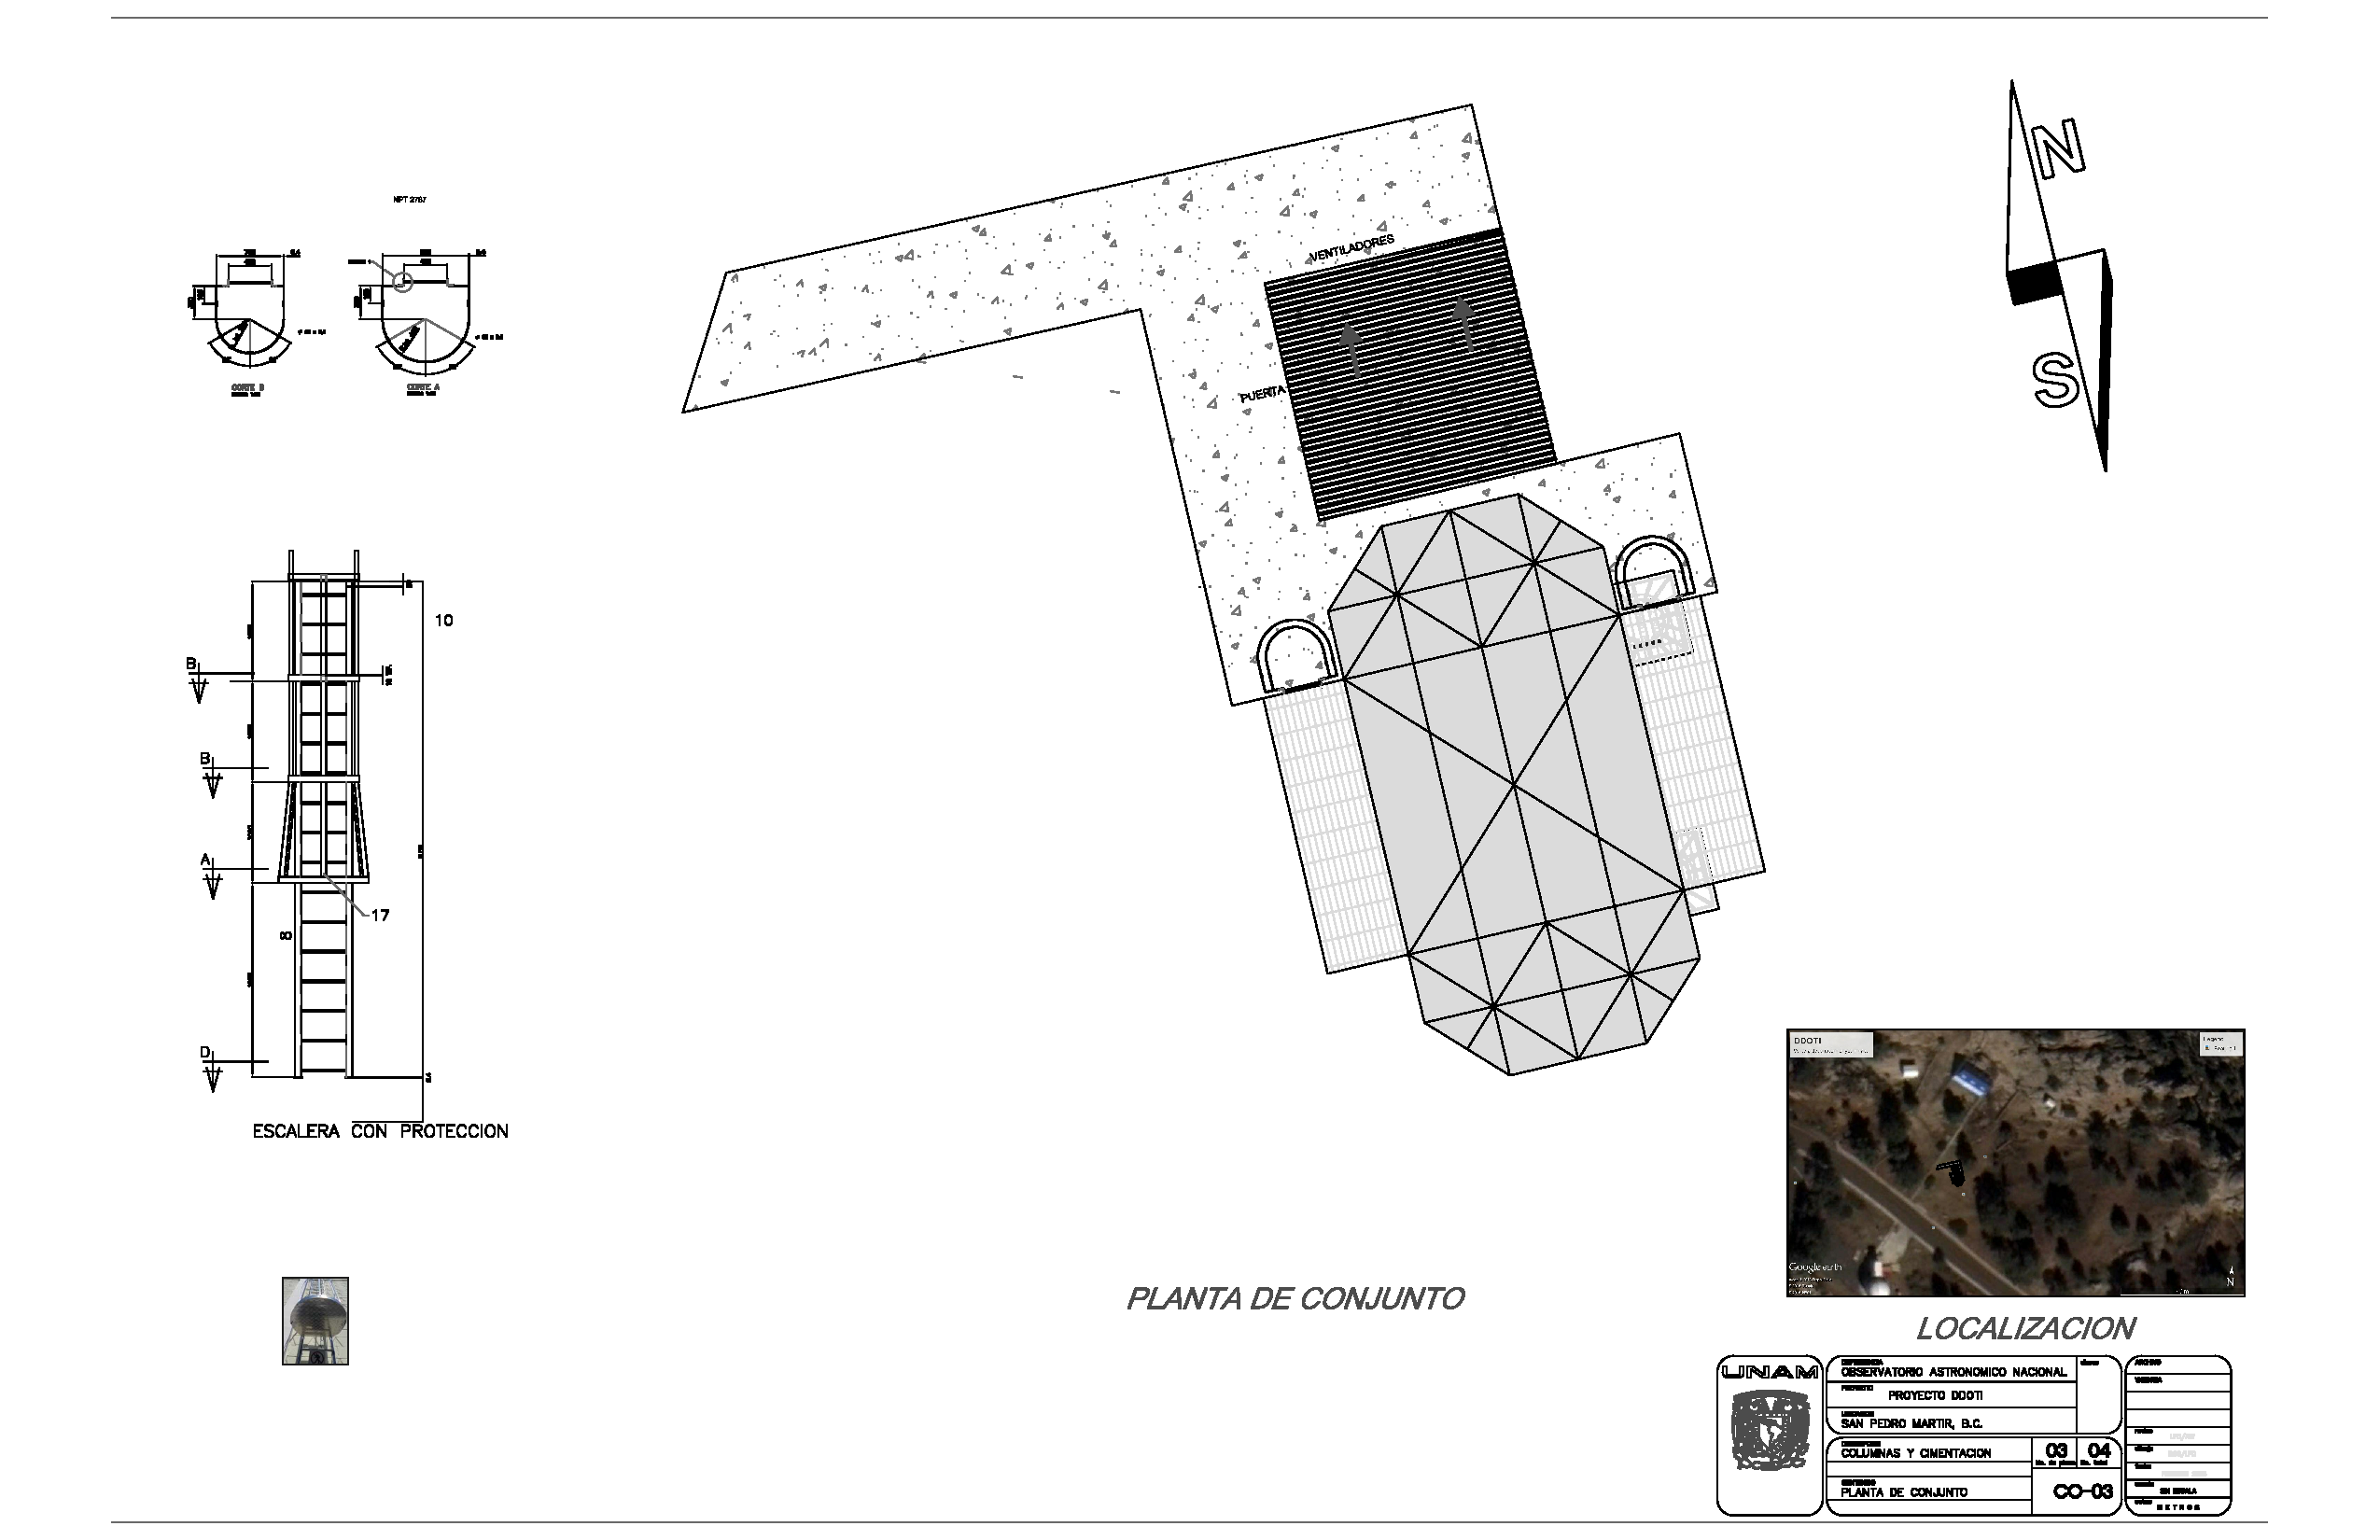
\includegraphics[height=0.8\linewidth,angle=90]{figures/buildings-ddoti-drawing-2016-2.pdf}
\end{center}
\caption{{\projectname} original 2016 design drawing (2 of 3). Note that the actual installation is rotated approximately 22 degrees east of the orientation shown here.}
\label{figure:buildings-drawing-2016-2}
\end{figure*}

\begin{figure*}
\begin{center}
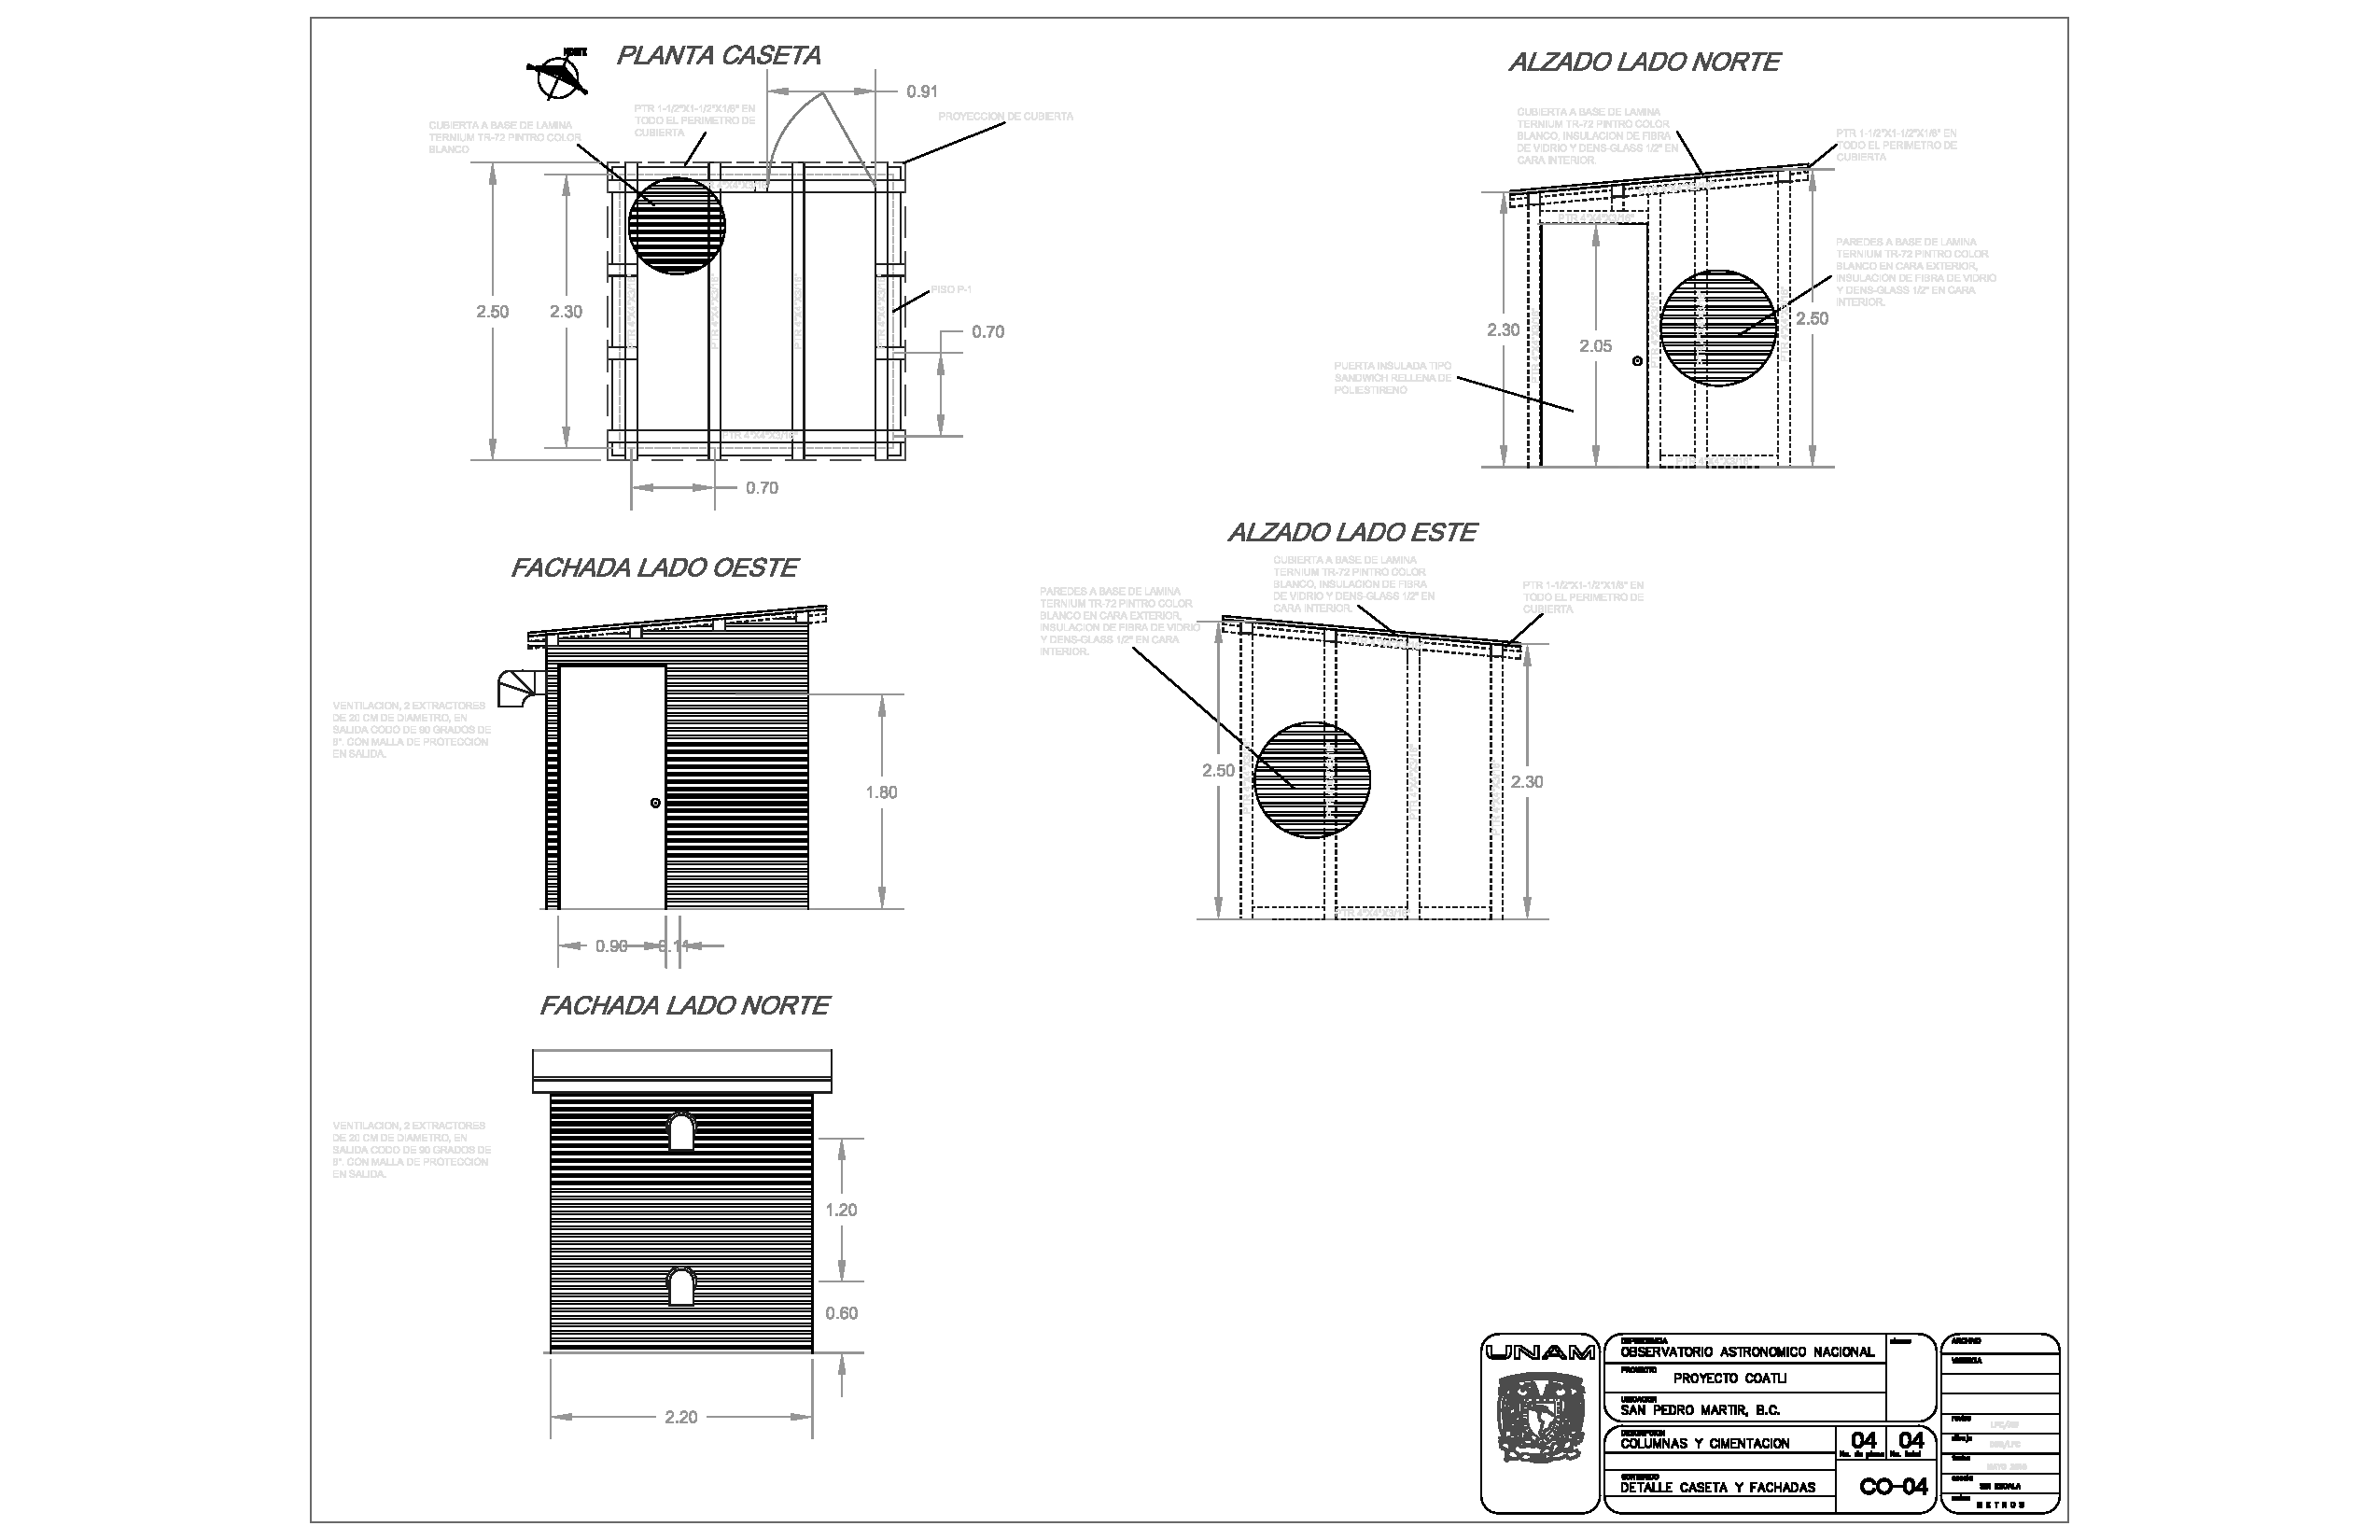
\includegraphics[height=0.95\linewidth,angle=90]{figures/buildings-ddoti-drawing-2016-3.pdf}
\end{center}
\caption{{\projectname} original 2016 design drawing (3 of 3).}
\label{figure:buildings-drawing-2016-3}
\end{figure*}

\begin{figure*}
\begin{center}
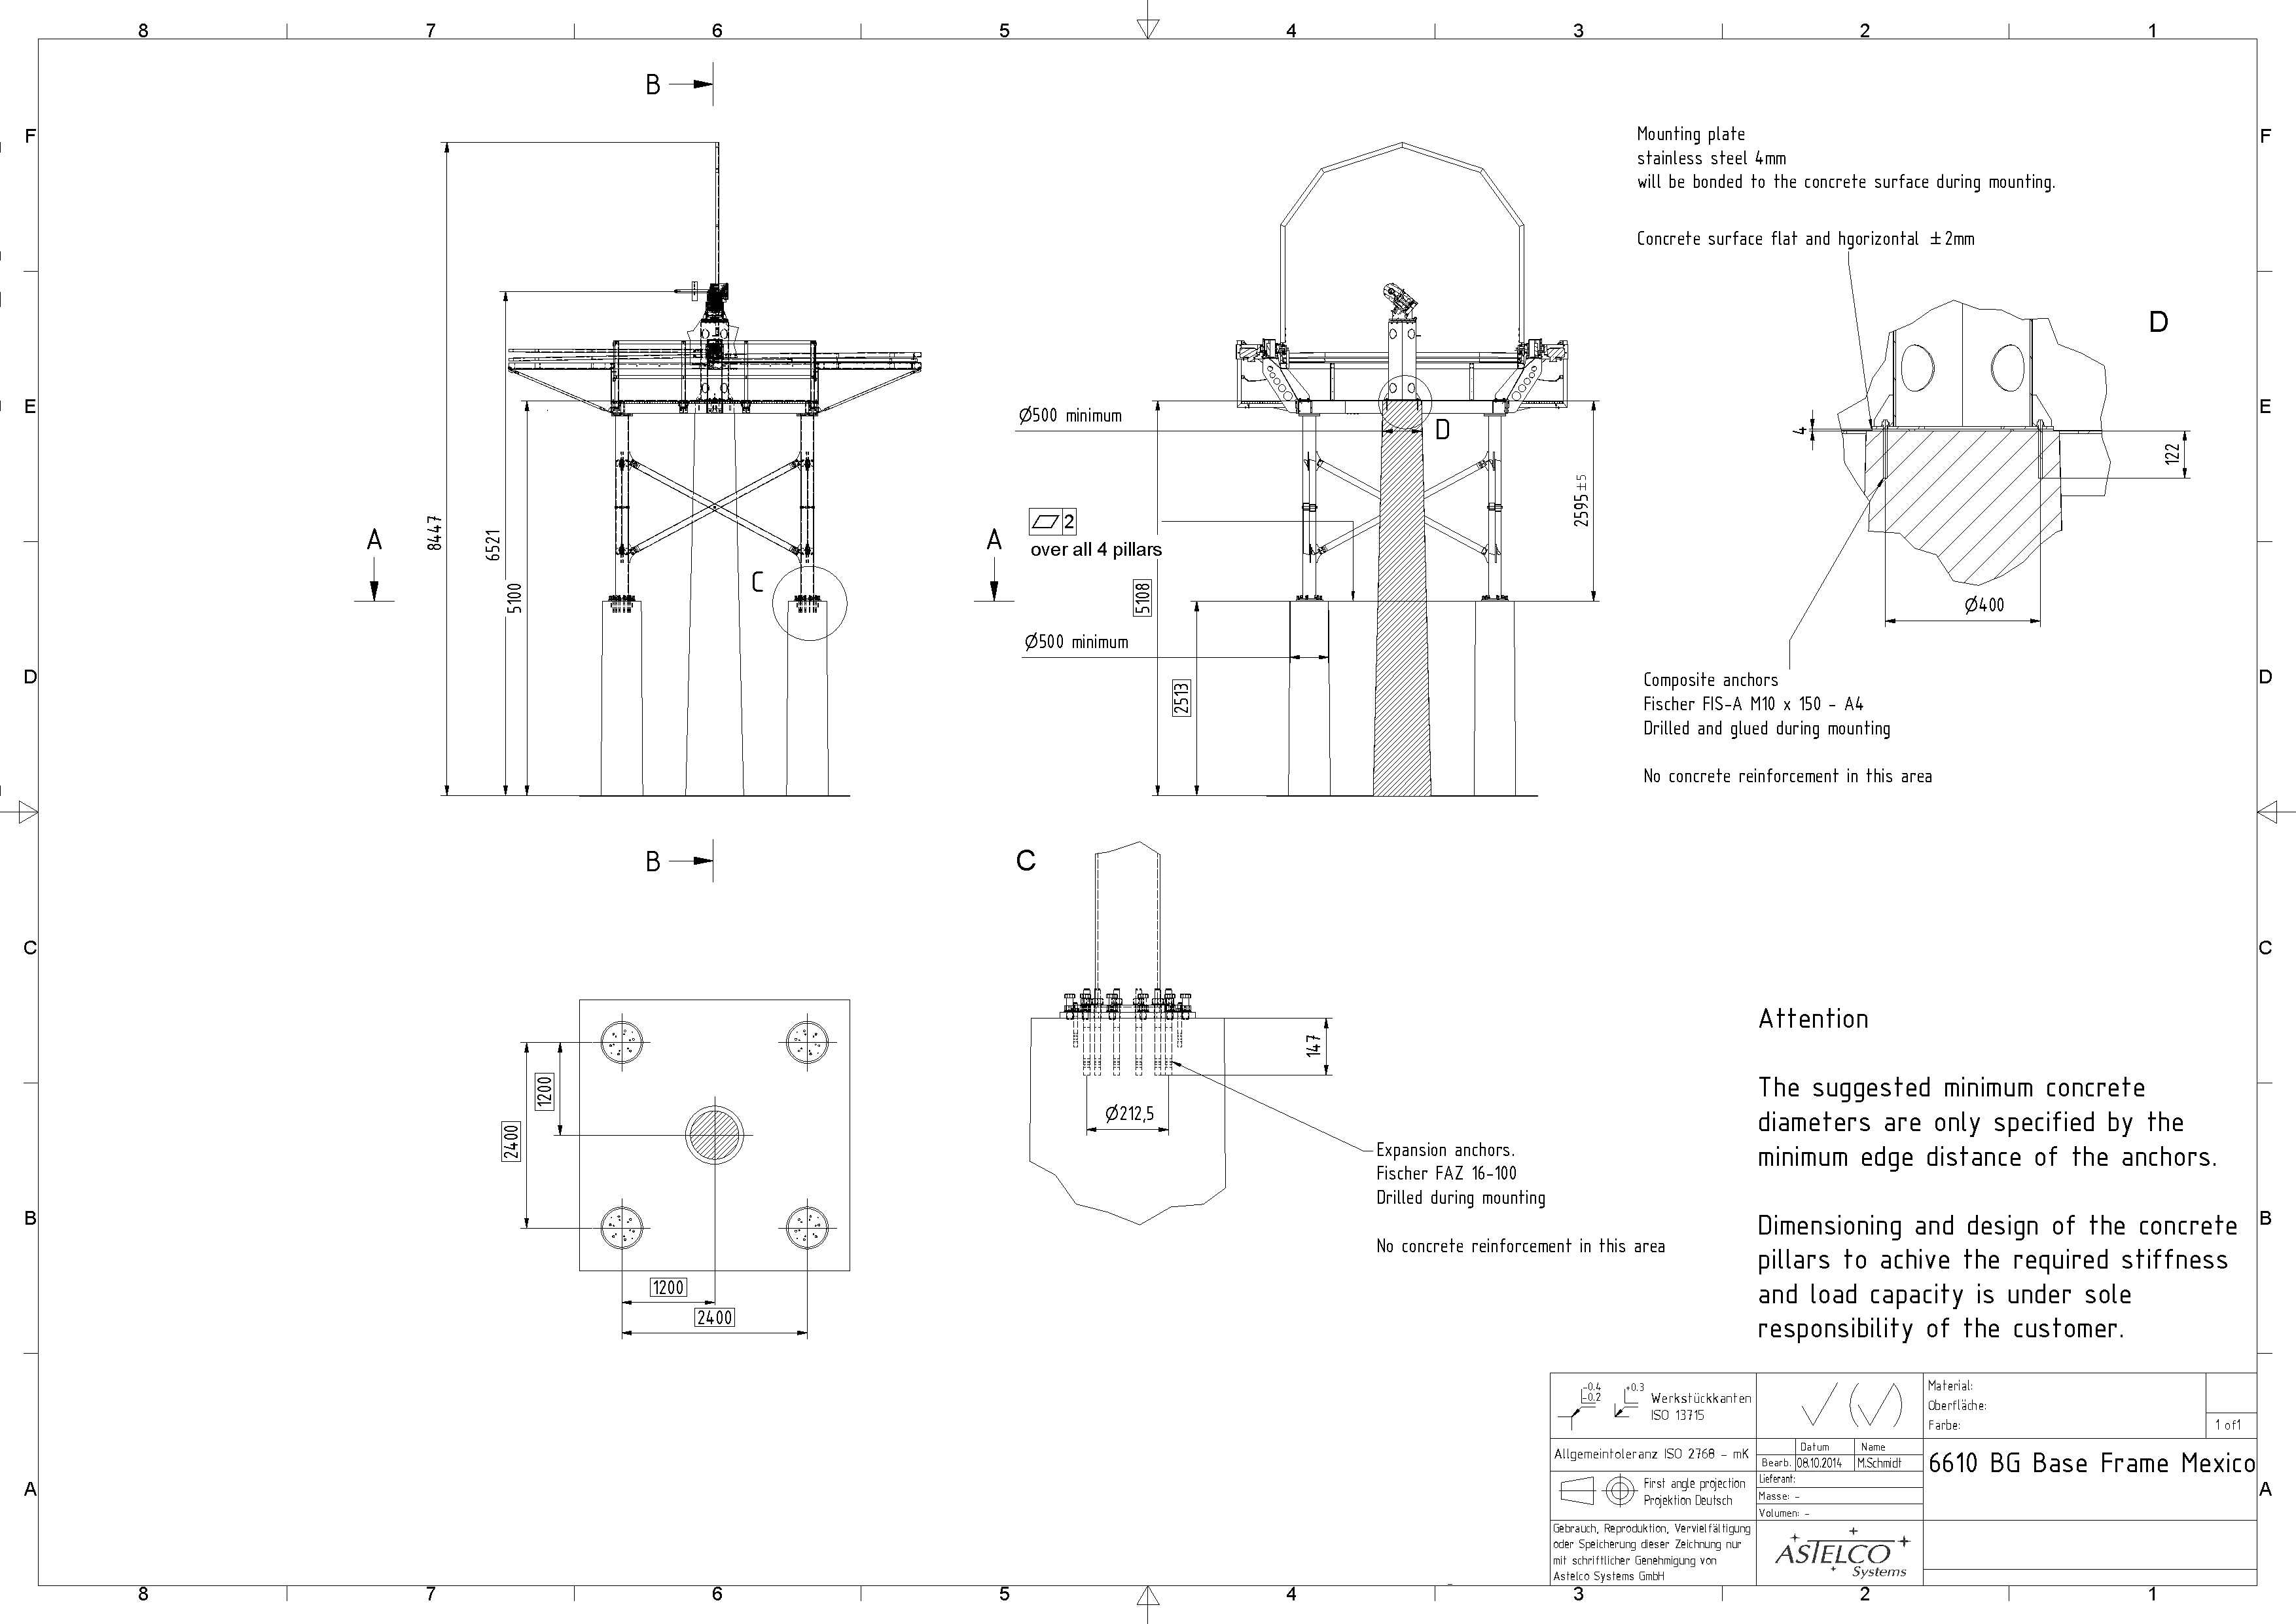
\includegraphics[height=0.95\linewidth,angle=90]{figures/buildings-ddoti-astelco-enclosure-drawing-6610}
\end{center}
\caption{{\projectname} ASTELCO platform and telescope pier (for COATLI).}
\label{figure:buildings-drawing-astelco}
\end{figure*}

\begin{figure*}
\begin{center}
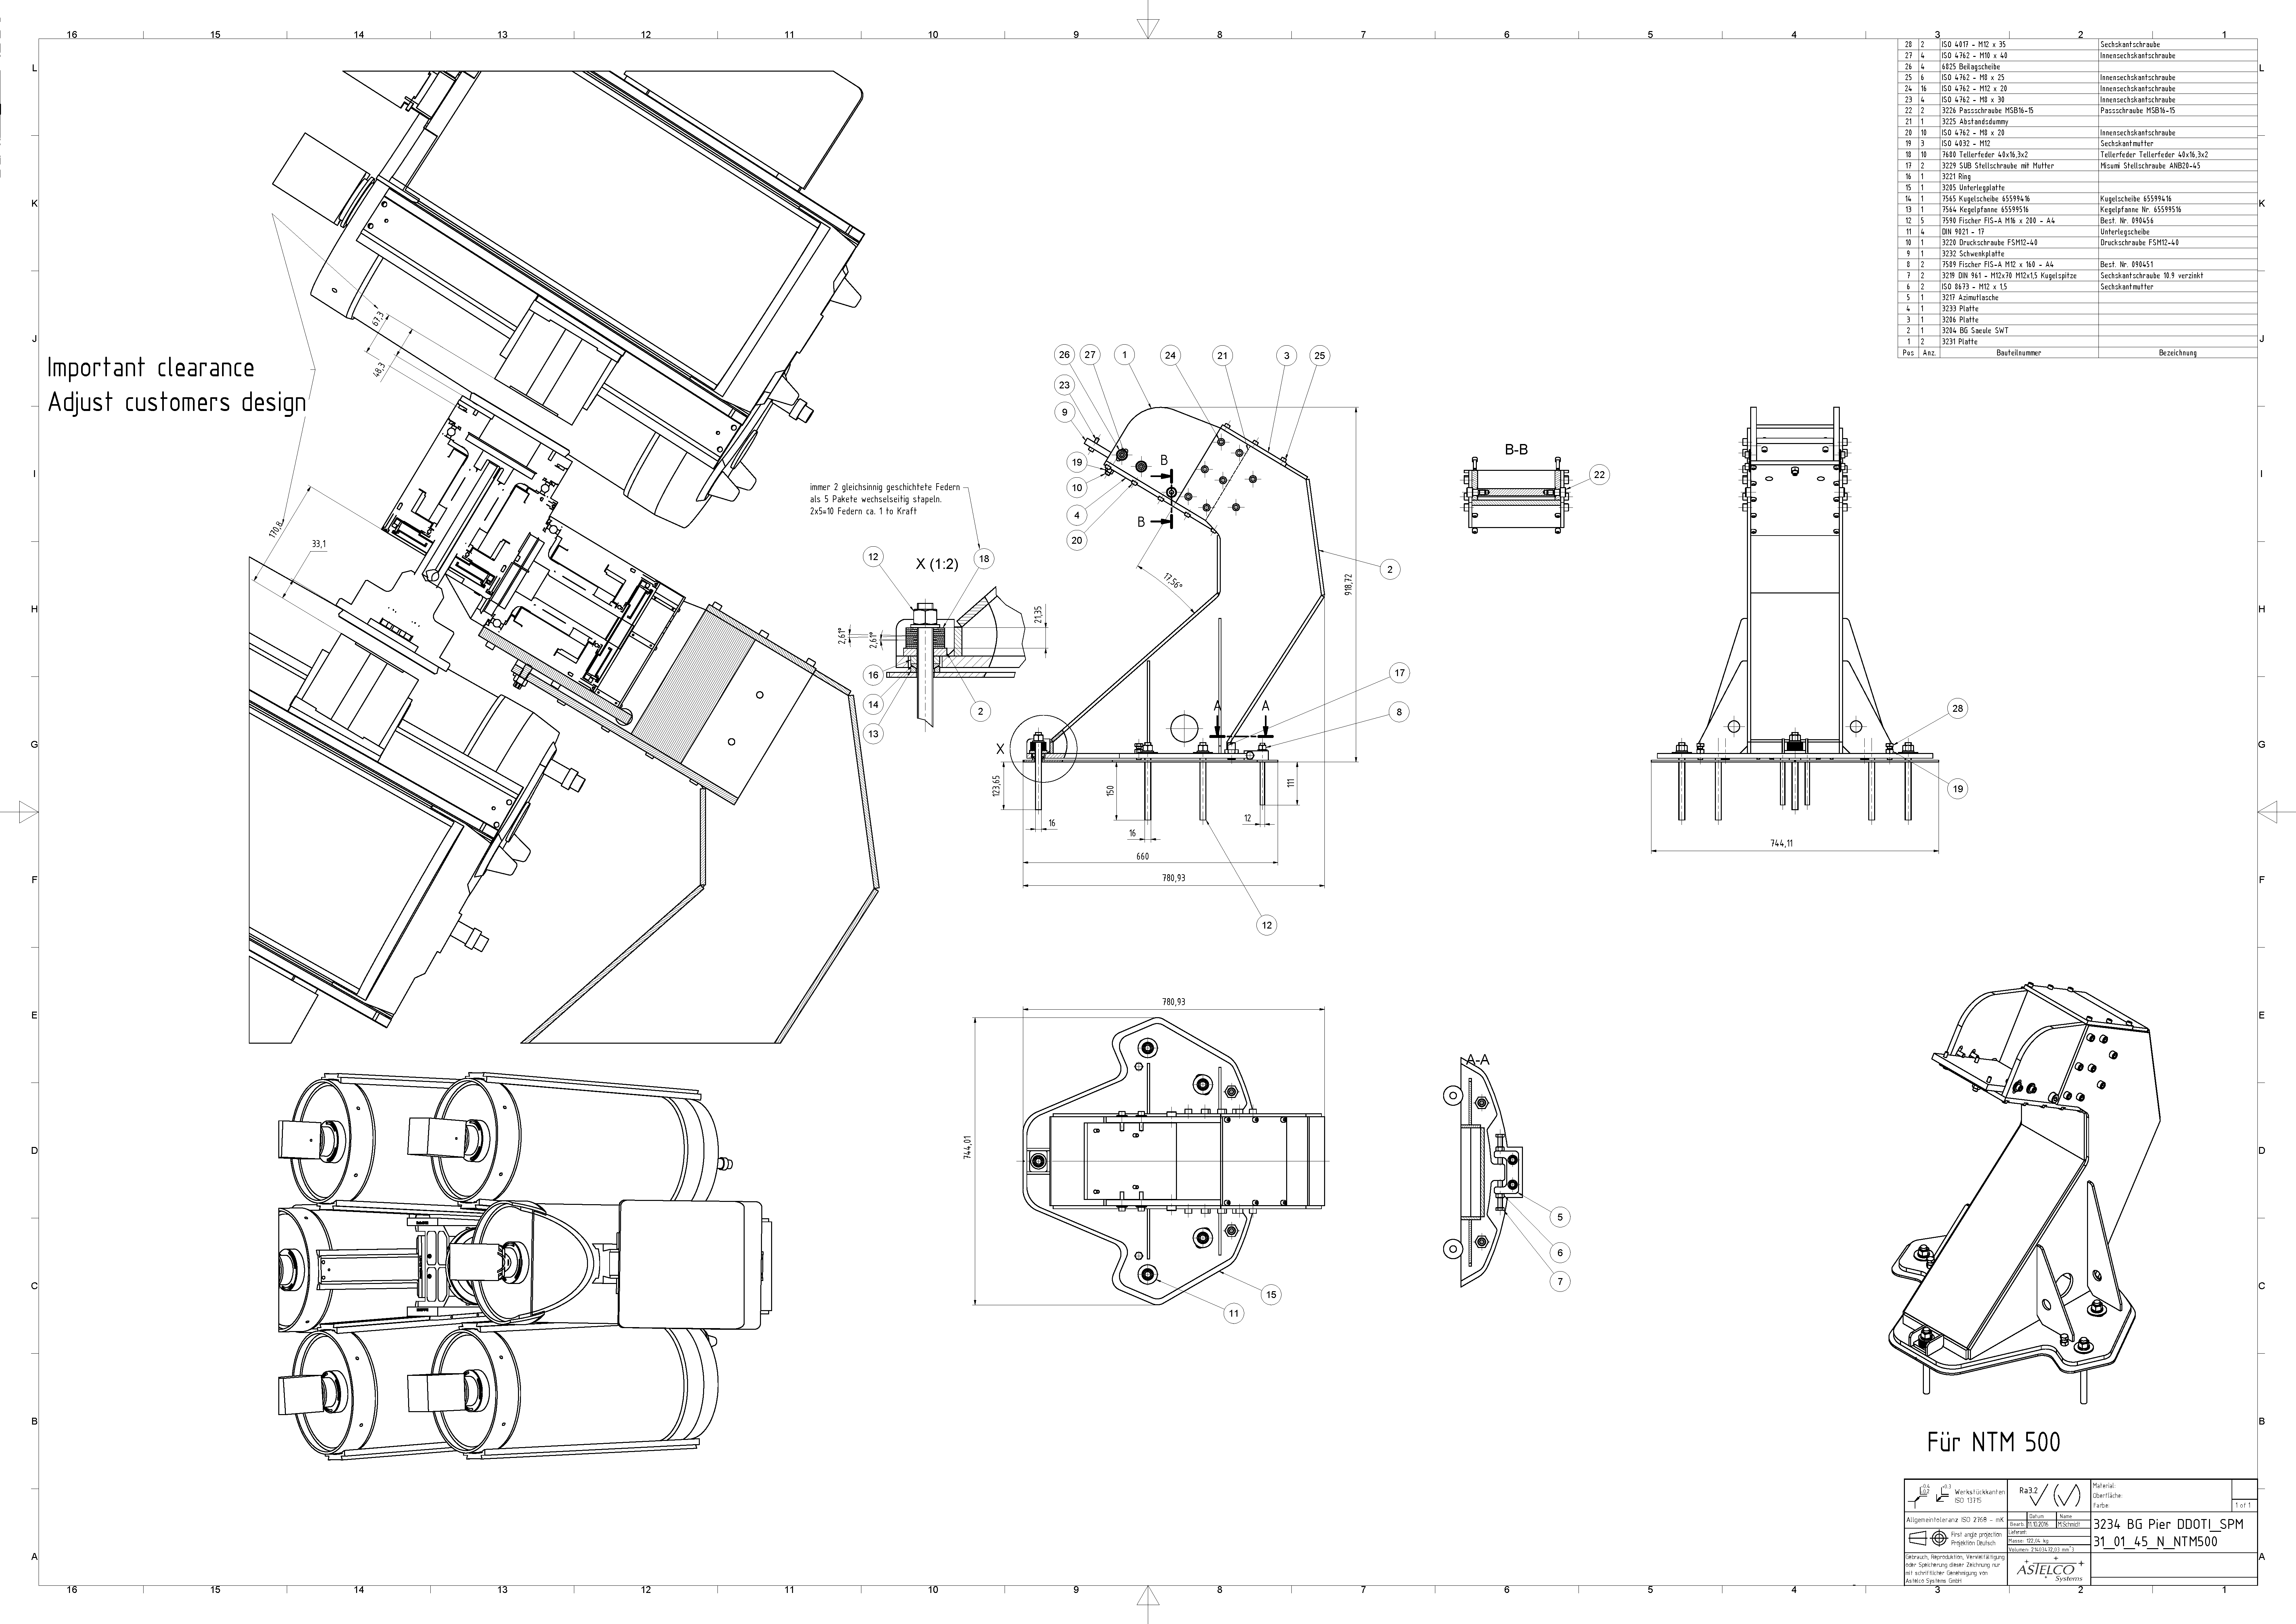
\includegraphics[height=0.95\linewidth,angle=90]{figures/buildings-ddoti-astelco-pier-drawing-3234}
\end{center}
\caption{{\projectname} ASTELCO pier.}
\label{figure:buildings-drawing-astelco-pier}
\end{figure*}

\fi

\section{Ground-Floor of the 84-cm Telescope Building}

We use the ground-floor of the 84-cm telescope building for storage of equipment and as a temporary work space.

{\projectname} tools and equipment are stored mainly in the equipment cabinet. They are to be used only for maintenance of COATLI and DDOTI and must be returned to the cabinet at the end of the maintenance procedure.

ASTELCO tools and equipment are stored in a locked metal box and are only to be used under the supervision of project or ASTELCO personnel.

\section{Shed}
\label{section:shed}
\label{section:shed-key}

The shed contains infrastructure and control electronics.

\begin{figure*}
\begin{center}
\begin{labeled}{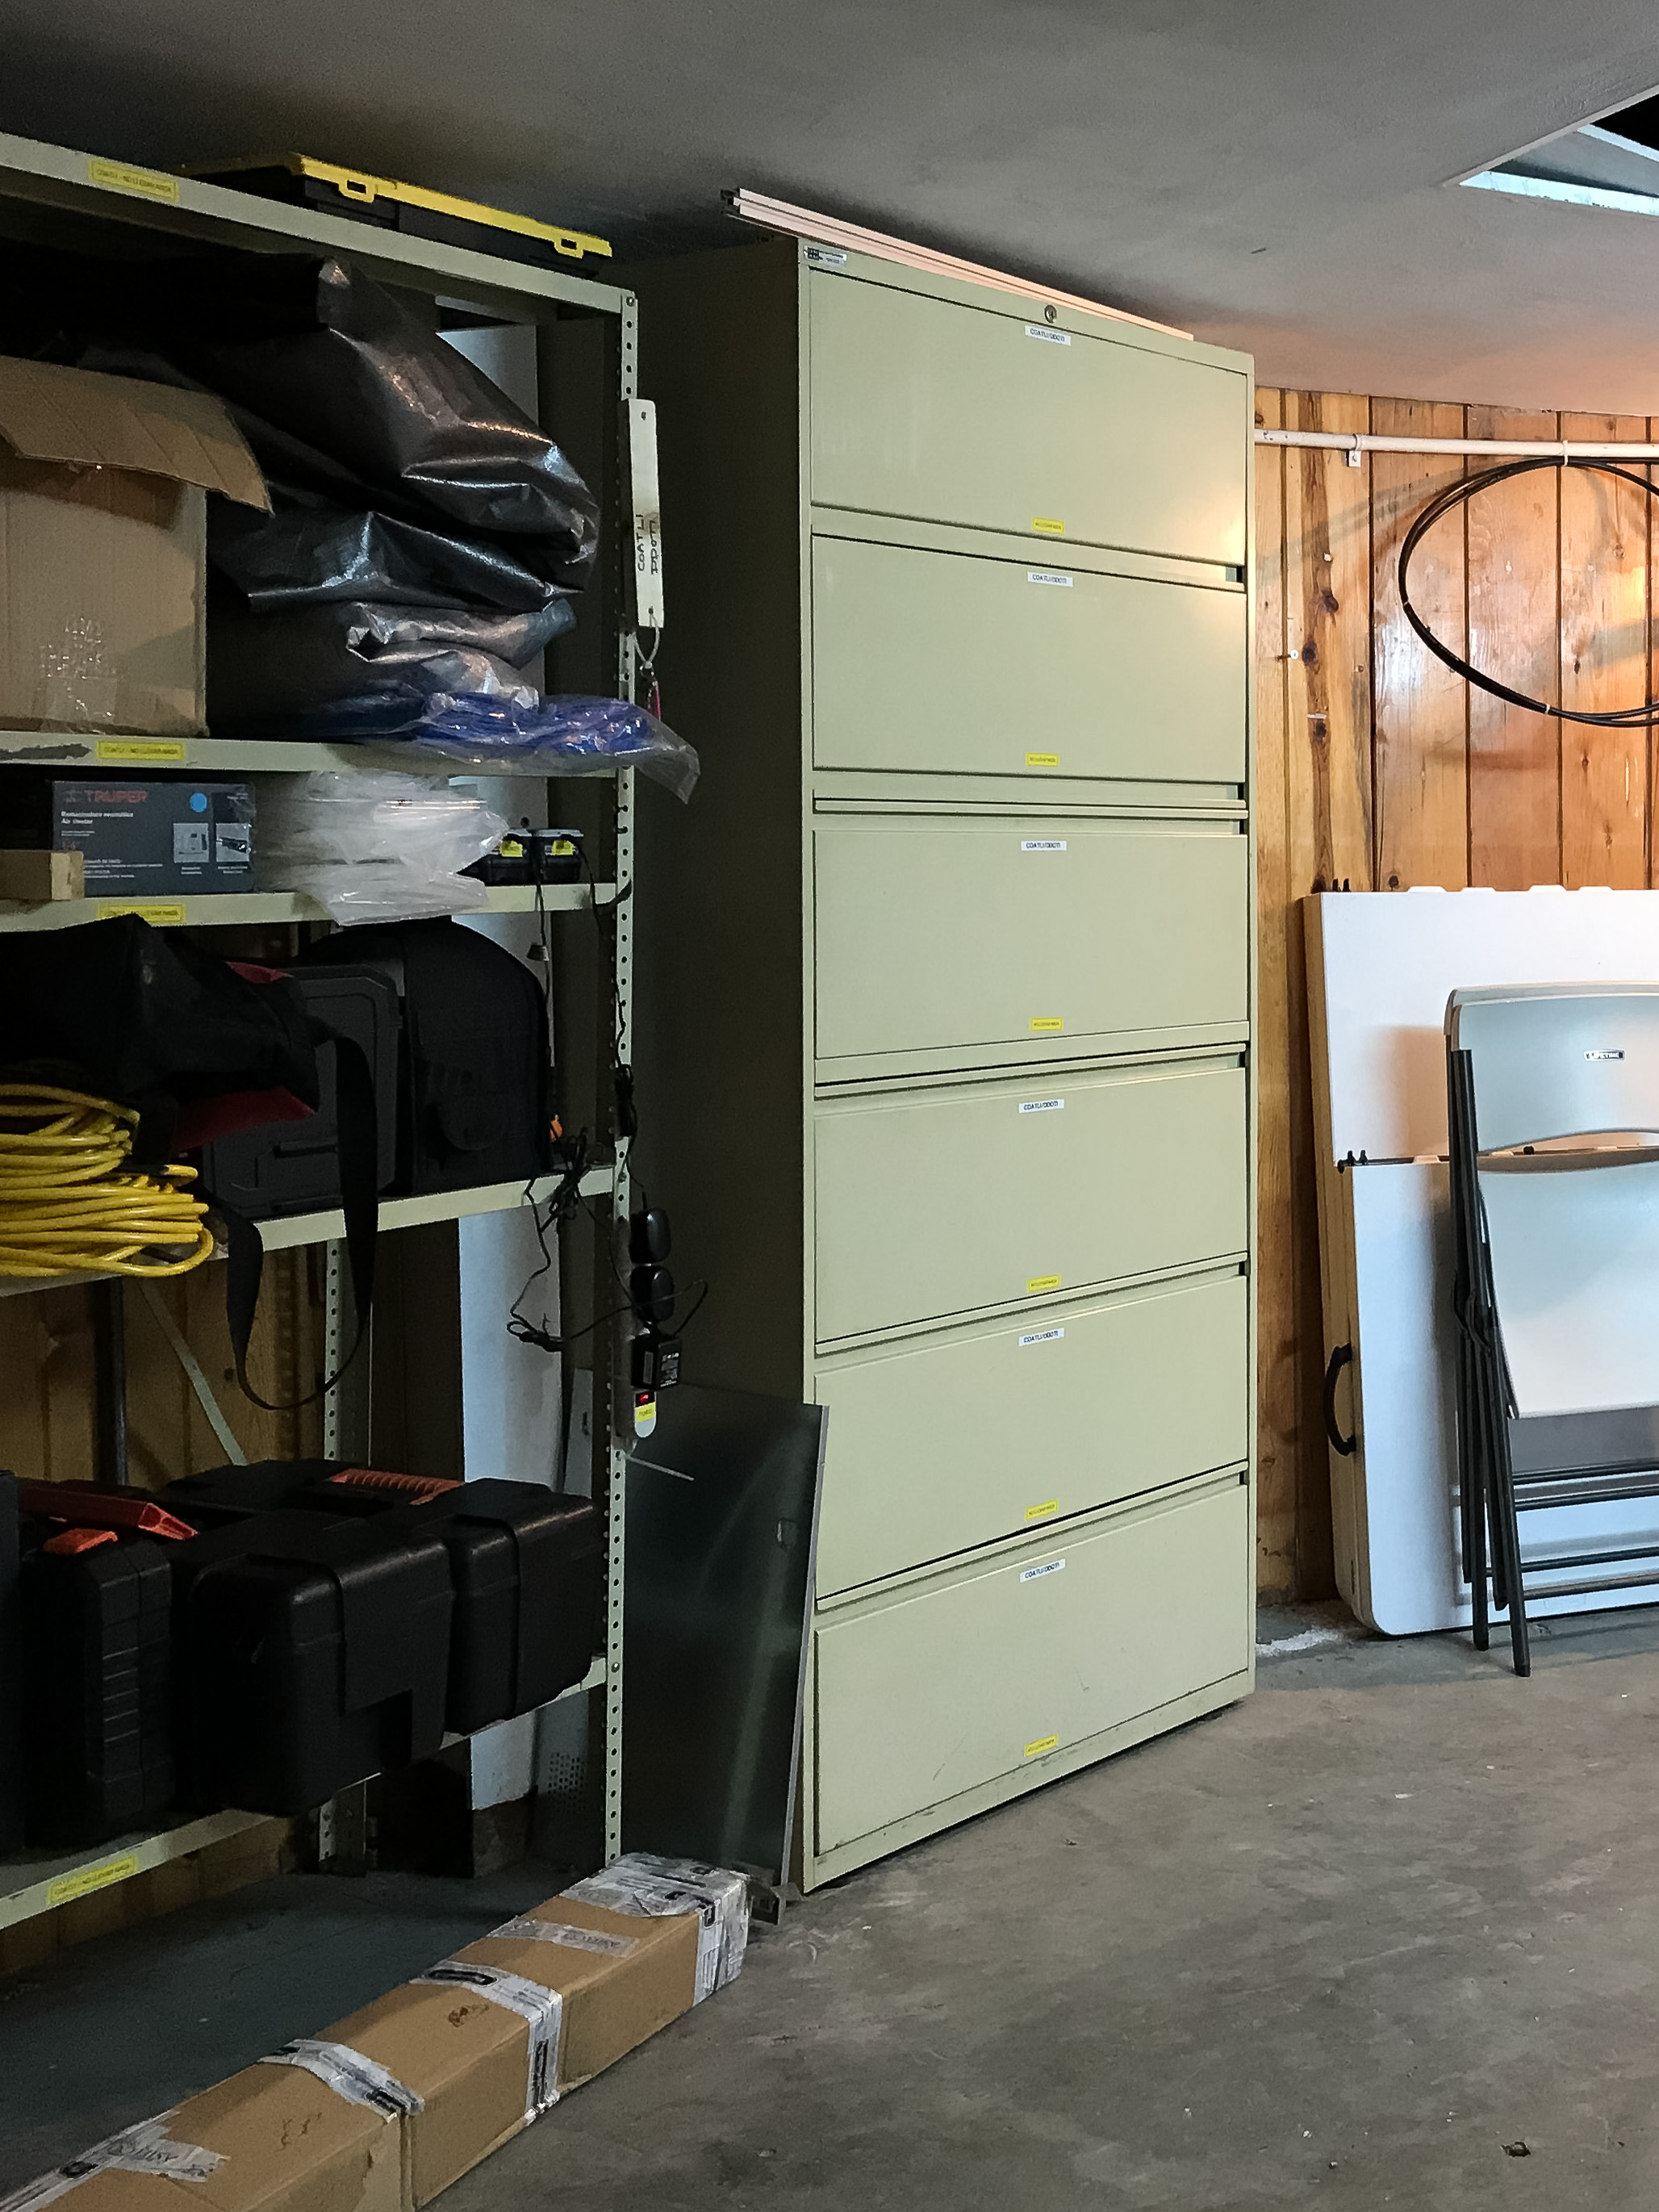
\includegraphics[width=0.8\linewidth]{figures/buildings-shed-key.jpg}}
\arrowandlabel{(-1,+3.5)}{(+0,+4)}{west}{Shed Key}
\end{labeled}
\end{center}
\caption{The shed key is hung on the shelves next to the cabinet in the ground floor of the 84-cm telescope building.}
\label{figure:buildings-shed-key}
\end{figure*}

The door to the shed should be left locked. 

The key should be hung on the shelves next to the cabinet in the ground-floor of the 84-cm telescope building (see Figure~\ref{figure:buildings-shed-key}).

The temperature in the shed it controlled by a heater and a pair of fans (one inlet and one exhaust). The fans are controlled by a Lux WIN100 thermostat and are set to turn on at 10 C. The internal thermostat of the heater is set to its minimum level.

%\section{Access Staircase and Walkways}

%\section{Tower, Platform, and Enclosure}

\section{Bibliography}

\begin{flushleft}
\begin{itemize}

\ifcoatlioan
\item “\href{bibliography/unam-coatli-building-drawing-2015-1.pdf}{Building 2015 Drawing 1 - Columns}”, UNAM.
\item “\href{bibliography/unam-coatli-building-drawing-2015-2.pdf}{Building 2015 Drawing 2 - Plan}”, UNAM.
\item “\href{bibliography/unam-coatli-building-drawing-2015-3.pdf}{Building 2015 Drawing 3 - Stairways}”, UNAM.
\item “\href{bibliography/unam-coatli-building-drawing-2015-4.pdf}{Building 2015 Drawing 4 - Shed}”, UNAM.
\item “\href{bibliography/unam-coatli-building-drawing-2015-5.pdf}{Building 2015 Drawing 5 - Location}”, UNAM.
\item “\href{bibliography/astelco-enclosure-drawing-0500}{ASTELCO Drawing 0500 -- Platform}”, ASTELCO.
\item “\href{bibliography/astelco-enclosure-drawing-5772}{ASTELCO Drawing 5572 -- Tower Mounting Plate}”, ASTELCO.
\item “\href{bibliography/astelco-enclosure-drawing-5772}{ASTELCO Drawing 5798 -- Tower}”, ASTELCO.
\item “\href{bibliography/astelco-enclosure-drawing-5772}{ASTELCO Drawing 6610 --  Tower, Platform, and Enclosure}”, ASTELCO.
\item “\href{bibliography/astelco-enclosure-drawing-5772}{ASTELCO Drawing 6658 -- Tower, Platform, and Enclosuure}”, ASTELCO.
\item “\href{bibliography/astelco-enclosure-drawing-5772}{ASTELCO Drawing 6662 -- Interface}”, ASTELCO.
\item “\href{bibliography/unam-coatli-building-drawing-2018-1.pdf}{Building 2018 Drawing 1 - Column}”, UNAM.
\item “\href{bibliography/unam-coatli-building-drawing-2018-2.pdf}{Building 2018 Drawing 2 - Floor Support Beams}”, UNAM.
\item “\href{bibliography/unam-coatli-building-drawing-2018-3.pdf}{Building 2018 Drawing 3 - Floor Support Beams}”, UNAM.
\fi

\ifddotioan
\item “\href{bibliography/unam-ddoti-building-drawing-2016-1.pdf}{Building 2016 Drawing 1 - Columns}”, UNAM.
\item “\href{bibliography/unam-ddoti-building-drawing-2016-2.pdf}{Building 2016 Drawing 2 - Plan and Location}”, UNAM.
\item “\href{bibliography/unam-ddoti-building-drawing-2016-3.pdf}{Building 2015 Drawing 3 - Shed}”, UNAM.
\item “\href{bibliography/astelco-enclosure-drawing-0500}{ASTELCO Drawing 0500 -- Platform}”, ASTELCO.
\item “\href{bibliography/astelco-enclosure-drawing-5772}{ASTELCO Drawing 5572 -- Tower Mounting Plate}”, ASTELCO.
\item “\href{bibliography/astelco-enclosure-drawing-5772}{ASTELCO Drawing 6610 --  Tower, Platform, and Enclosure}”, ASTELCO.
\item “\href{bibliography/astelco-enclosure-drawing-5772}{ASTELCO Drawing 6658 -- Tower, Platform, and Enclosuure}”, ASTELCO.
\item “\href{bibliography/astelco-enclosure-drawing-5772}{ASTELCO Drawing 6662 -- Interface}”, ASTELCO.
\item “\href{bibliography/astelco-ddoti-pier-drawing-3205}{ASTELCO Drawing 3205 -- Pier Mounting Plate}”, ASTELCO.
\item “\href{bibliography/astelco-ddoti-pier-drawing-3205}{ASTELCO Drawing 3234 -- Pier}”, ASTELCO.
\fi

\item “\href{bibliography/lux-win100-manual}{Lux WIN100 Manual}”, Lux.

\end{itemize}
\end{flushleft}
